\documentclass[12pt]{article}

\usepackage{geometry}
 \geometry{
 a4paper,
 total={170mm,257mm},
 left=10mm,
 right=10mm,
 top=10mm,
 bottom=20mm,
 headheight=75pt
 }
% \usepackage[utf8x]{inputenc}
\usepackage{fontspec}
\setmainfont{Open Sans}
\setsansfont{Noto Sans}
\usepackage{graphicx}
\usepackage{forloop}
\usepackage{subcaption}
\usepackage{url}       % `\url`s
\usepackage{floatrow}
\usepackage{hyperref}
\usepackage{cleveref}
\graphicspath{{resources_CAD/}}





\newcommand\pic[1]{(\cref{#1})} %Где нужно сослаться на рисунок

\hypersetup{
    colorlinks=true,
    linkcolor=blue,
    urlcolor=cyan,
    }

% The preamble ends with the command \begin{document}
\newcounter{themenumber}
\newcounter{thenumberr}
\begin{document}

% Global variant 1
\begin{center}
    \LARGE <<Introduction to Mechanical Engineering>> \\ \textbf{Final Exam} \\ \textit{CAD modeling} \\ Variant: 9
\end{center}
\begin{enumerate}
    \item Make all CAD models from the blueprints, which provided below \pic{fig:t11,fig:t12}. (15 score)
    \item Make an assembly. Description is on the figure \pic{fig:resources_CAD/global_var1/h2.png}. (5 score)
     
    Decimal number --- <3 first surname letters>$2023.$<variant>$.000$ (Bulichev $\rightarrow$ $BUL2023.09.000$) 
    \item  Make the same blueprints (without dimensions), based on your CAD models. (3 extra score)
    \item  Provide a BOM for your assembly. It should contain name, decimal number, material, amount of details. (2 extra score)
\end{enumerate}

\begin{figure}[H]
    \begin{subfigure}{0.49\textwidth}
        \centering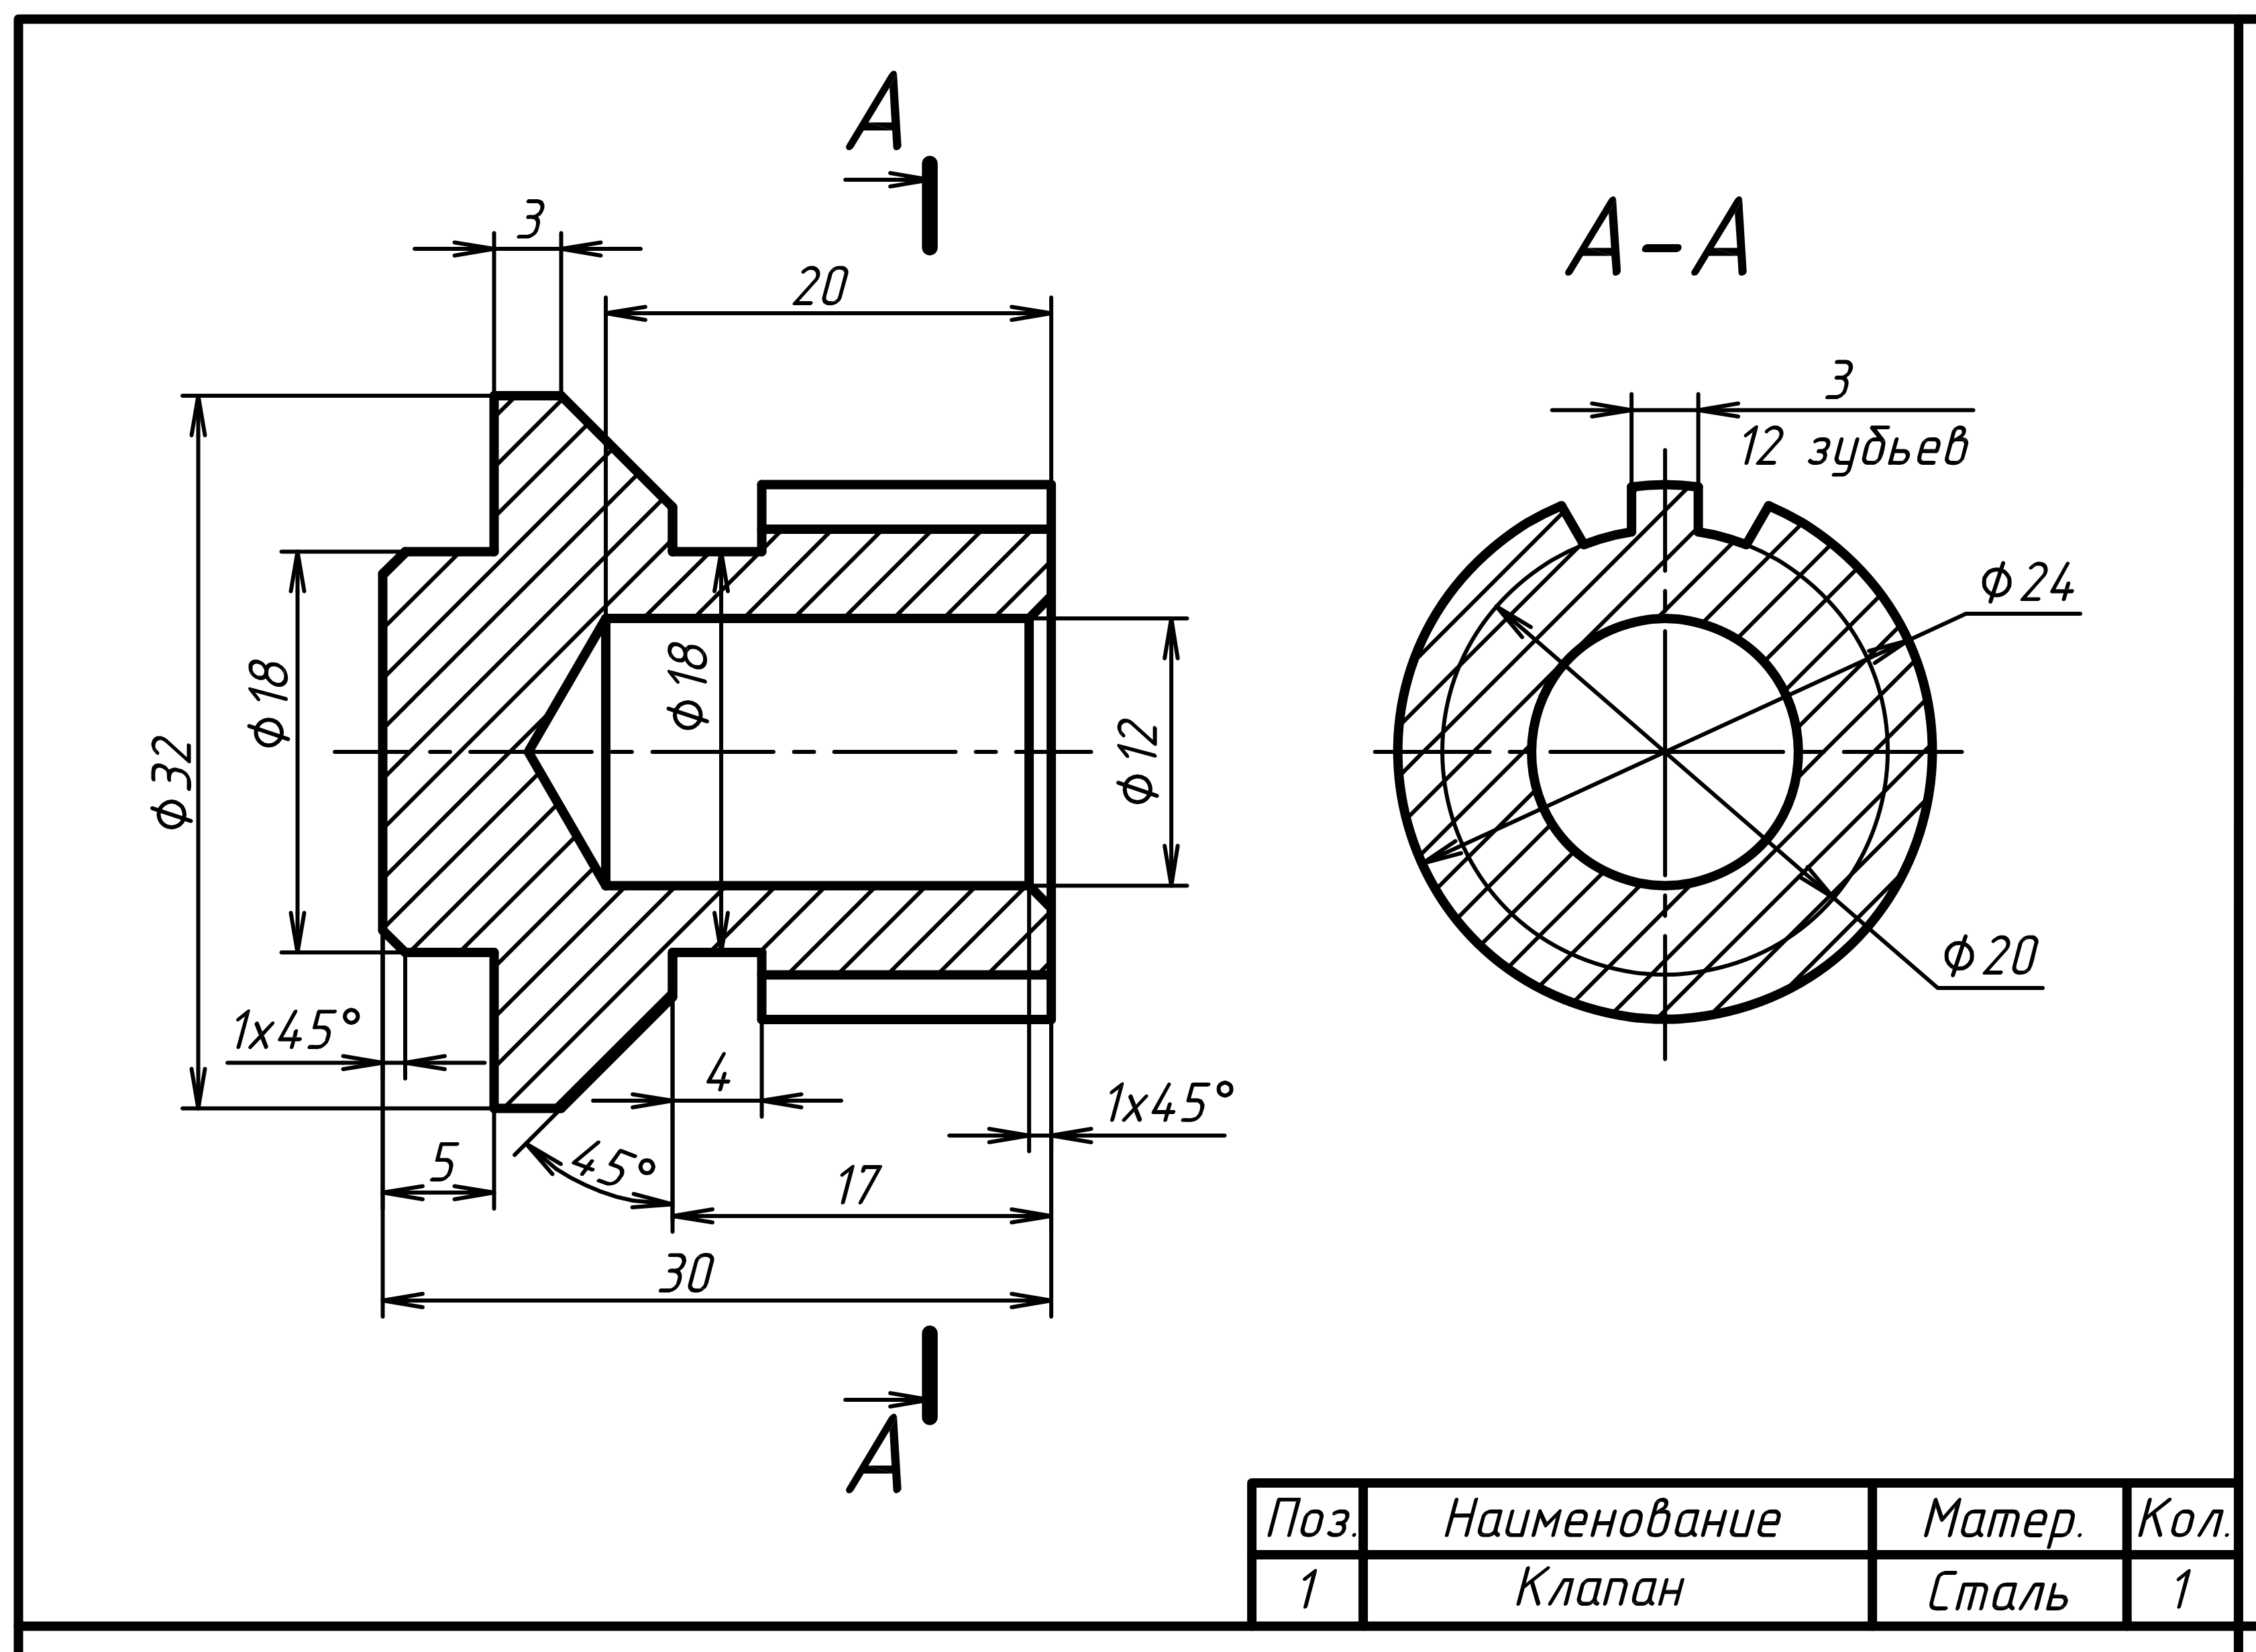
\includegraphics[height=8cm,width=1\textwidth,keepaspectratio]{resources_CAD/global_var1/t1.png}
        \caption{Part 1}
        \label{fig:resources_CAD/global_var1/t1.png}
    \end{subfigure}
    \begin{subfigure}{0.49\textwidth}
        \centering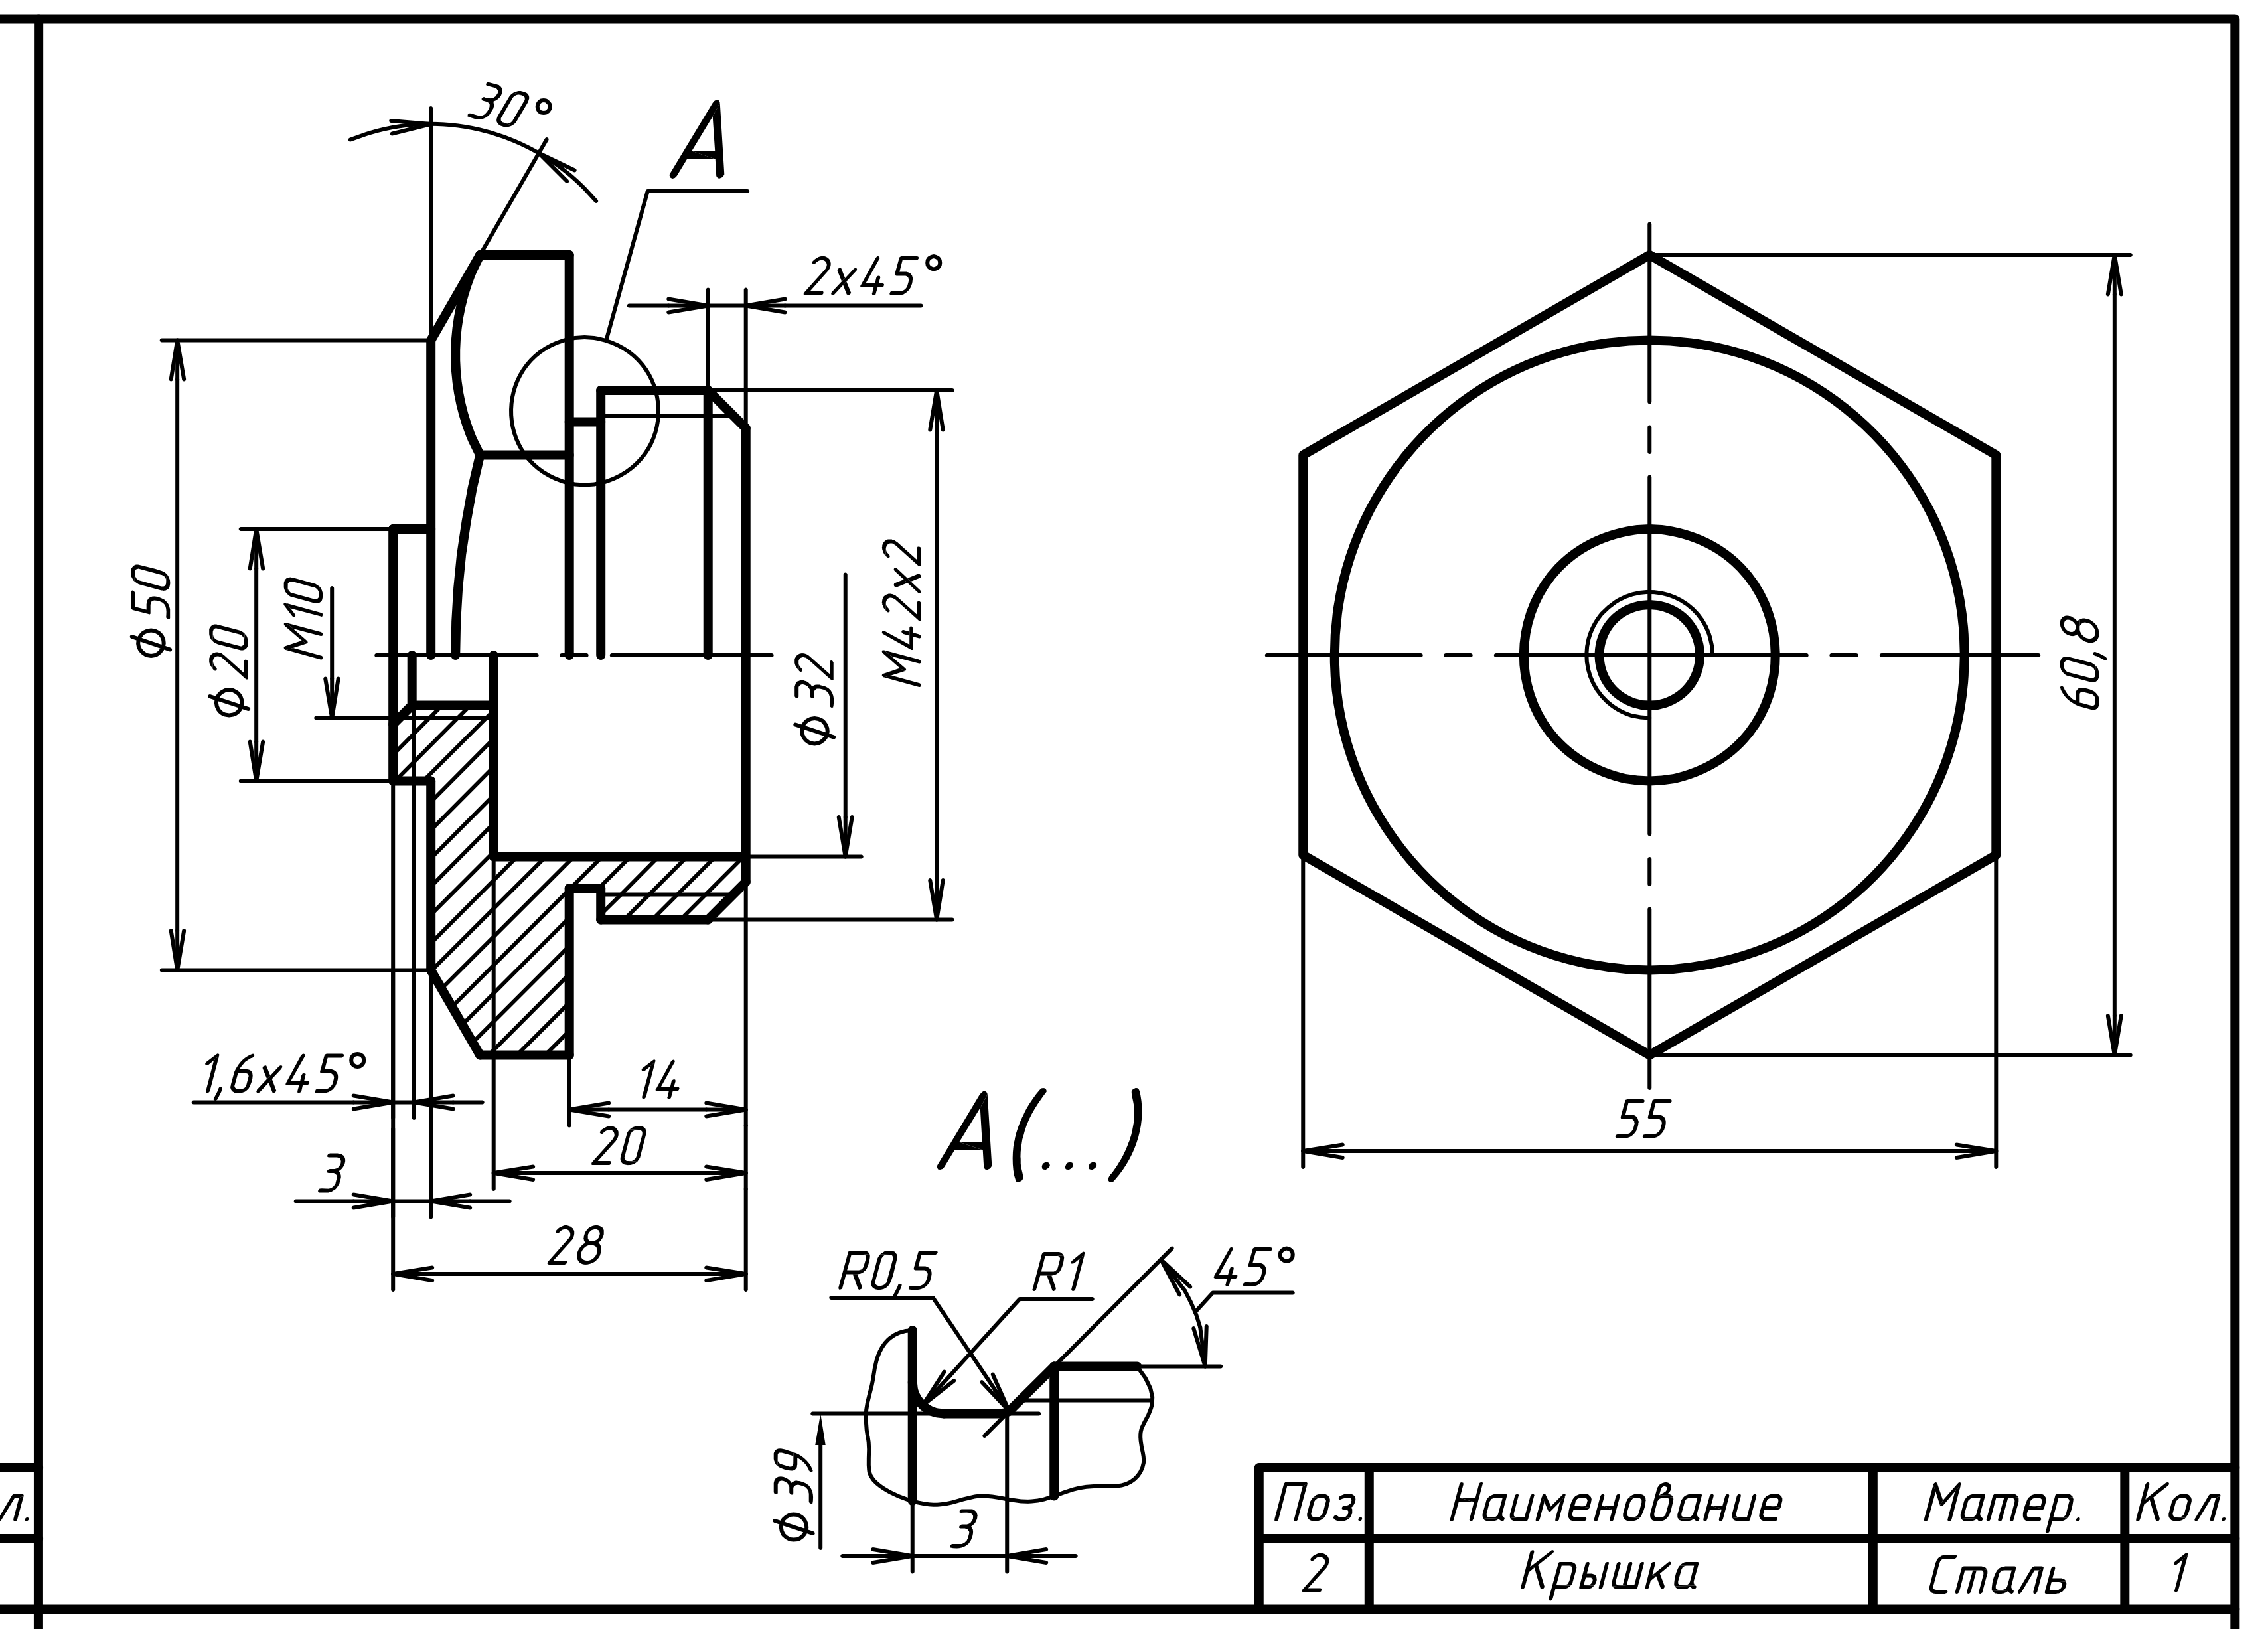
\includegraphics[height=8cm,width=1\textwidth,keepaspectratio]{resources_CAD/global_var1/t2.png}
        \caption{Part 2}
        \label{fig:resources_CAD/global_var1/t2.png}
    \end{subfigure}

    \begin{subfigure}{0.49\textwidth}
        \centering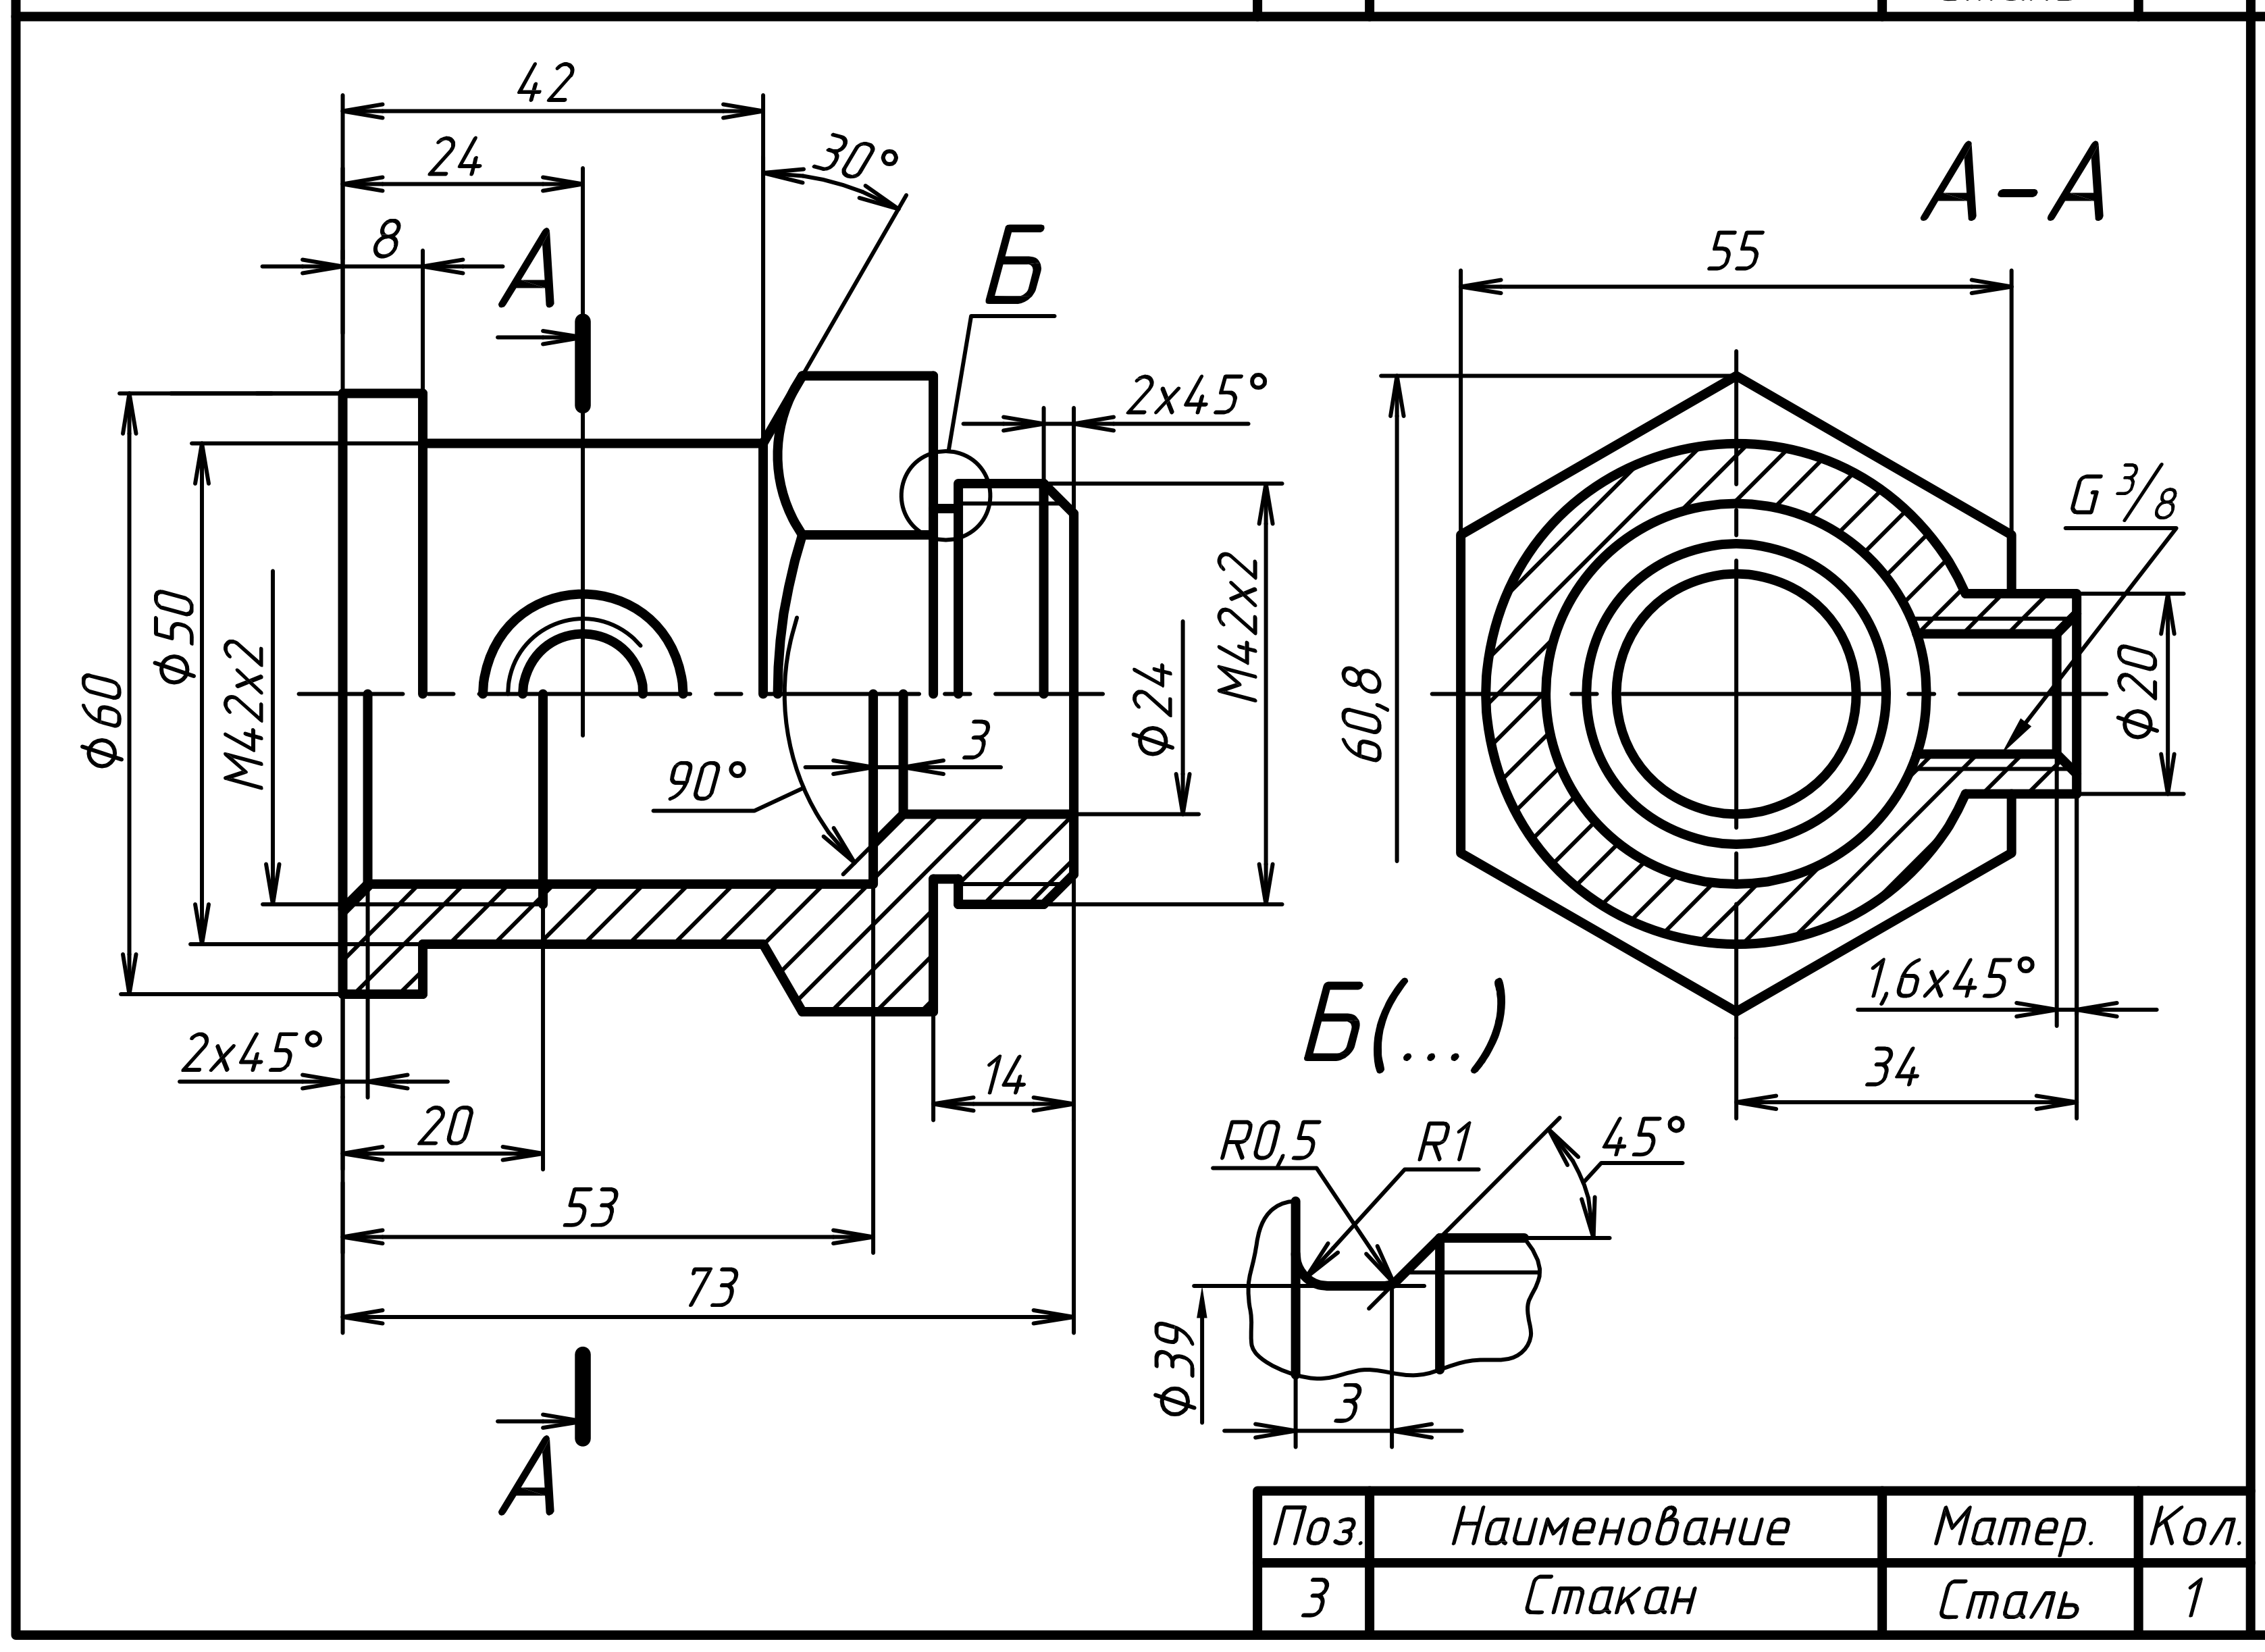
\includegraphics[height=8cm,width=1\textwidth,keepaspectratio]{resources_CAD/global_var1/t3.png}
        \caption{Part 3}
        \label{fig:resources_CAD/global_var1/t3.png}
    \end{subfigure}
    \begin{subfigure}{0.49\textwidth}
        \centering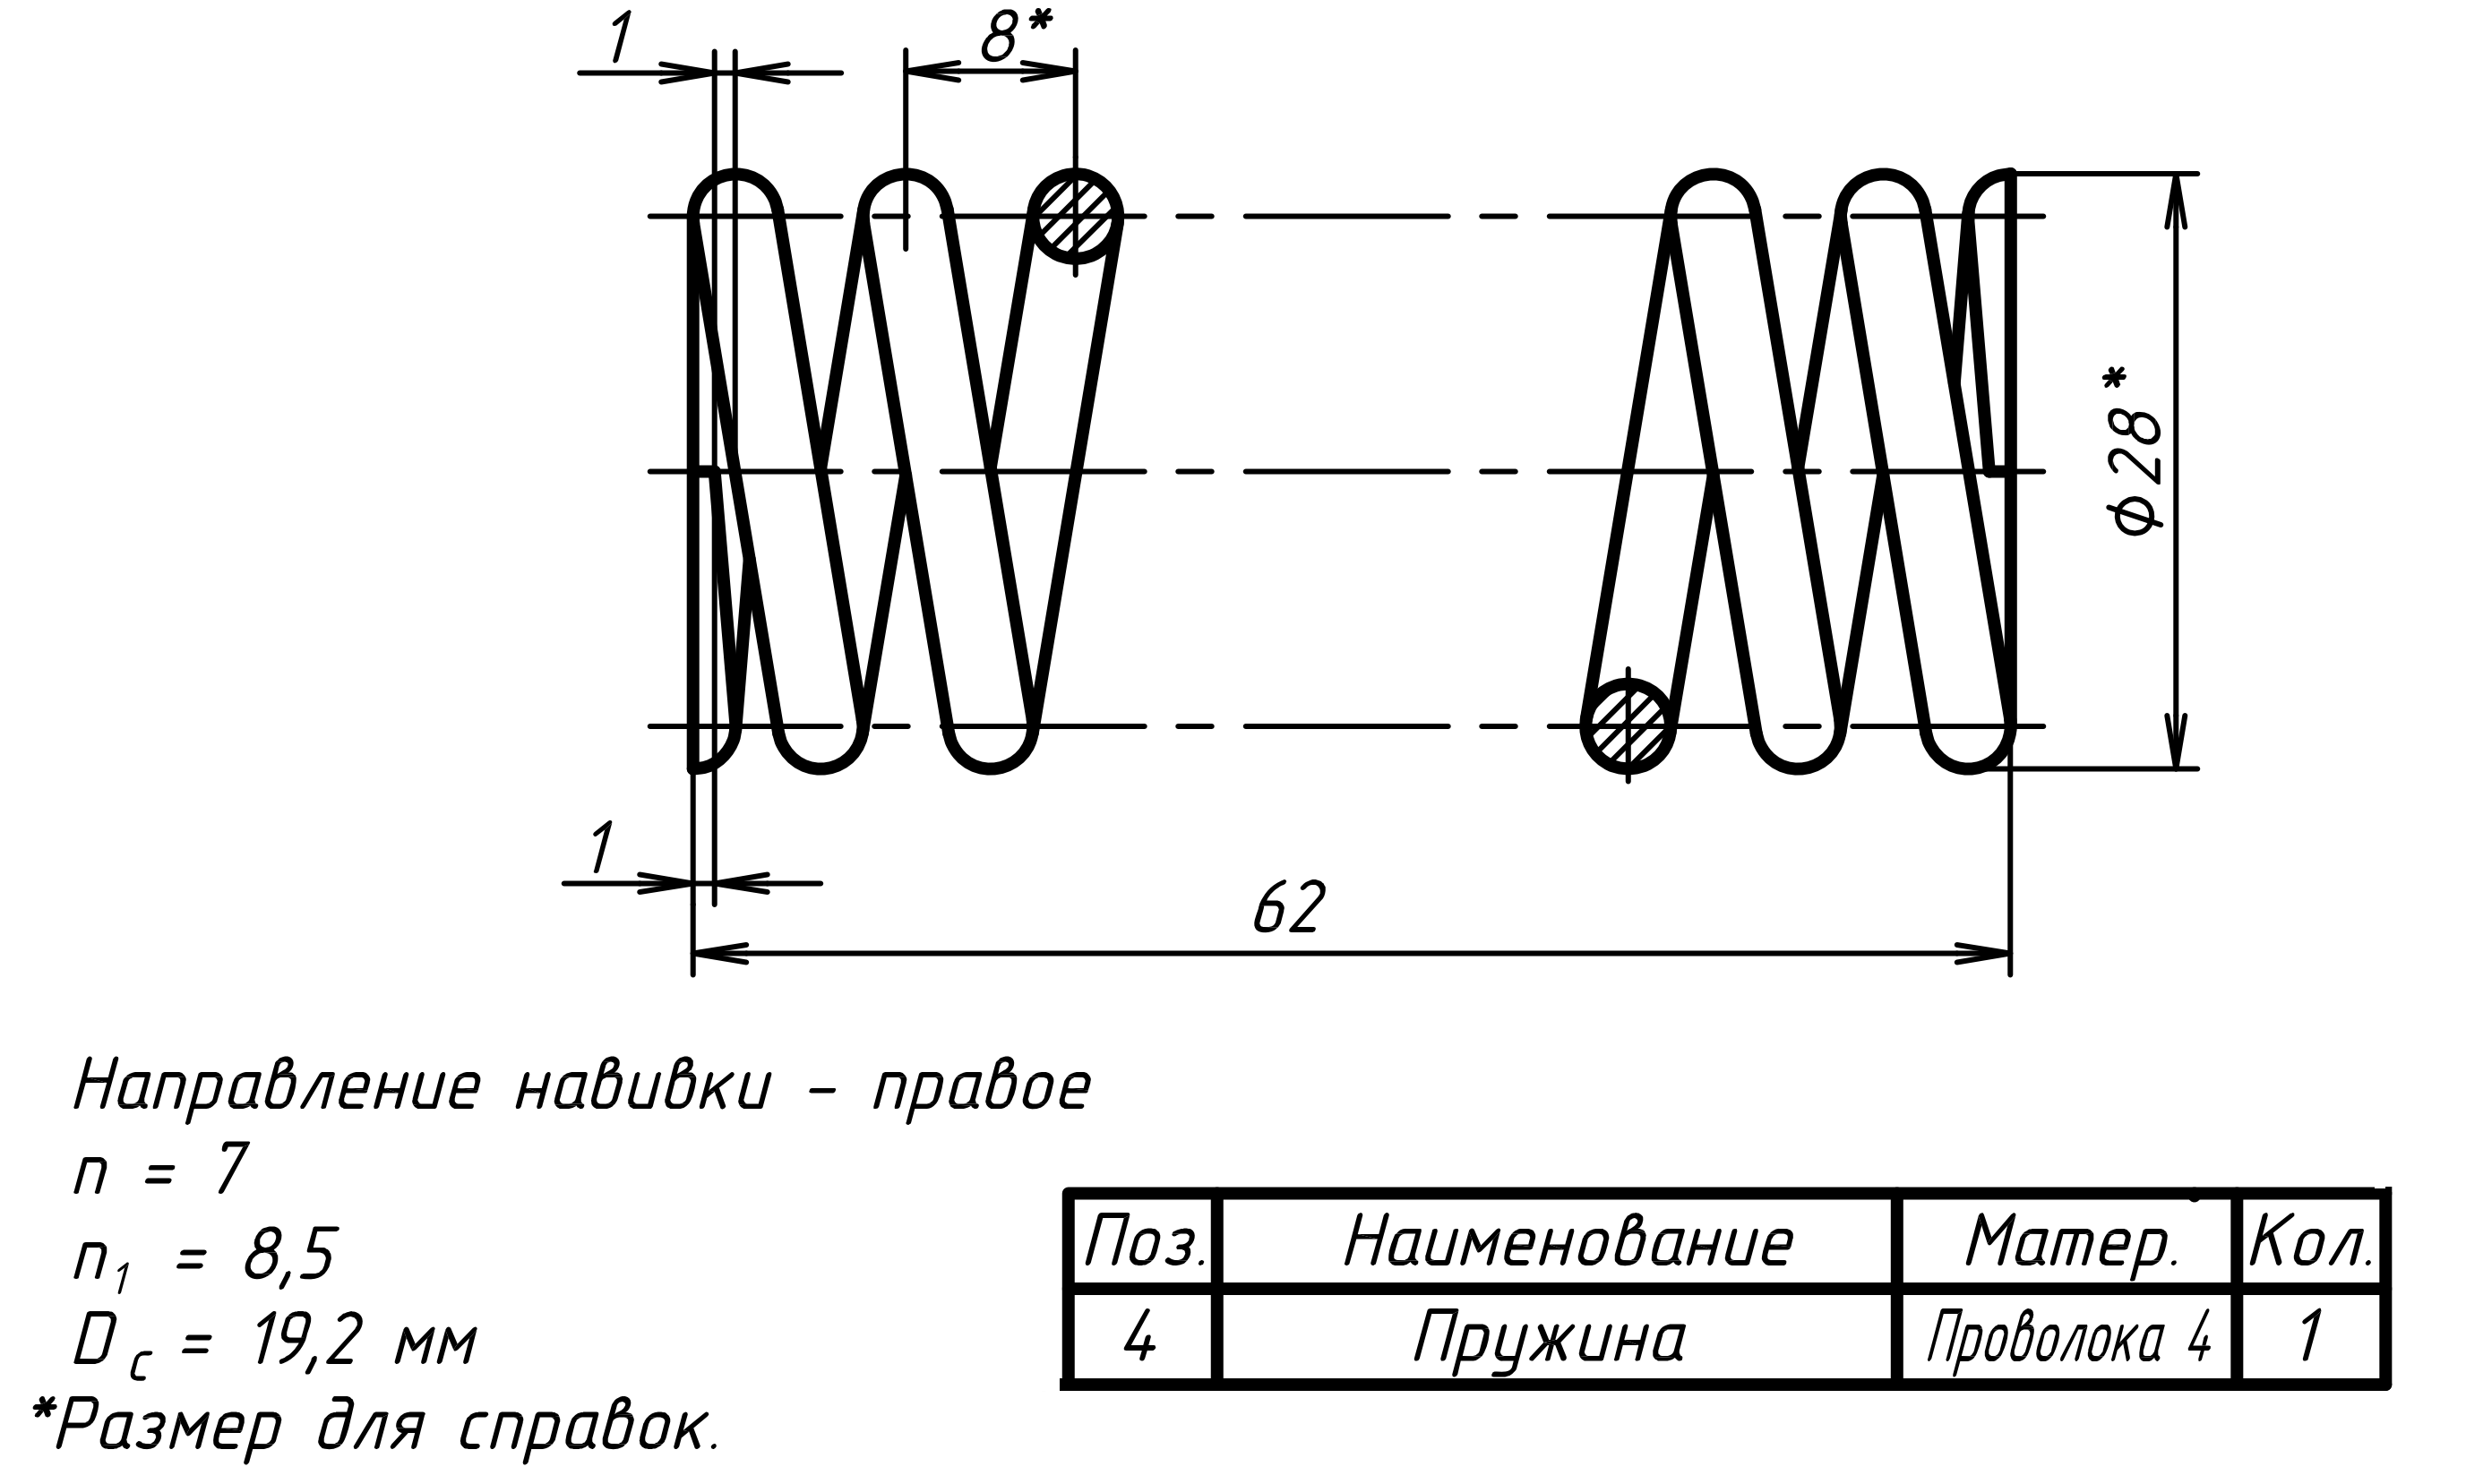
\includegraphics[height=8cm,width=1\textwidth,keepaspectratio]{resources_CAD/global_var1/t4.png}
        \caption{Part 4}
        \label{fig:resources_CAD/global_var1/t4.png}
    \end{subfigure}
\caption{Task 1}
\label{fig:t11}
\end{figure}

\begin{figure}[H]

    \begin{subfigure}[c]{0.59\textwidth}
        \centering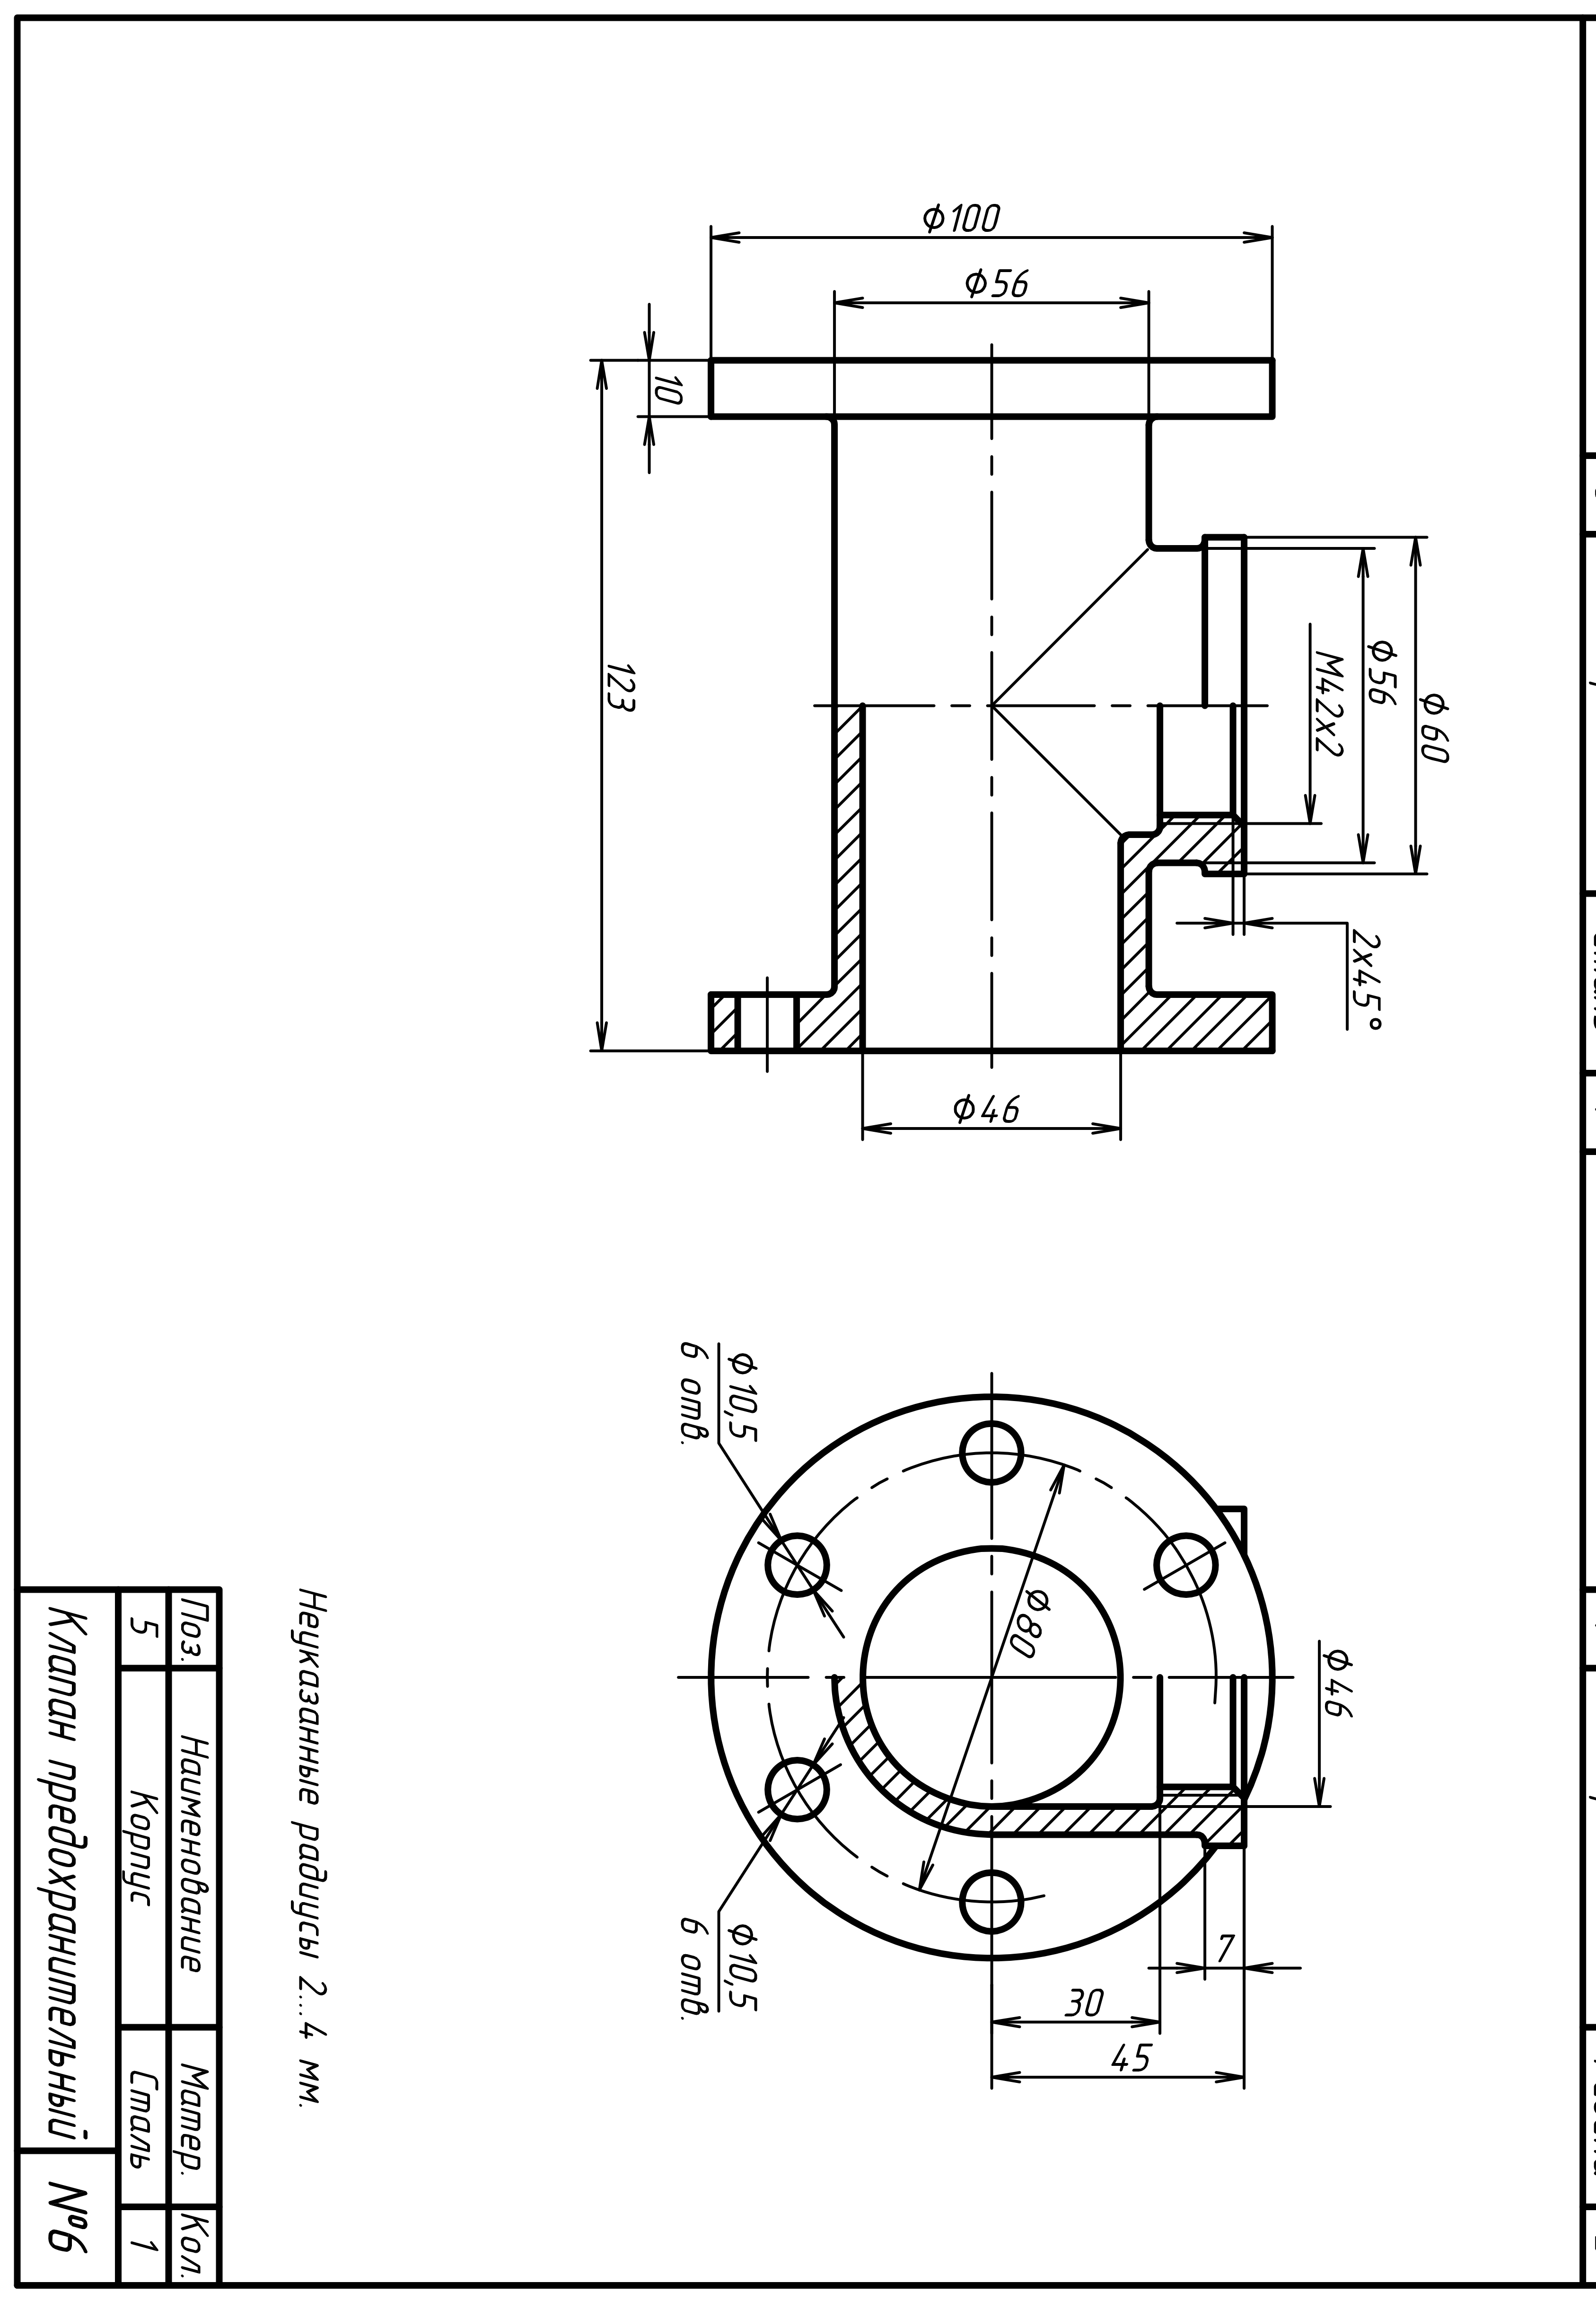
\includegraphics[height=8cm,width=1\textwidth,keepaspectratio]{resources_CAD/global_var1/t5.png}
        \caption{Part 5}
        \label{fig:resources_CAD/global_var1/t5.png}
    \end{subfigure}
    \begin{subfigure}[c]{0.39\textwidth}
        \centering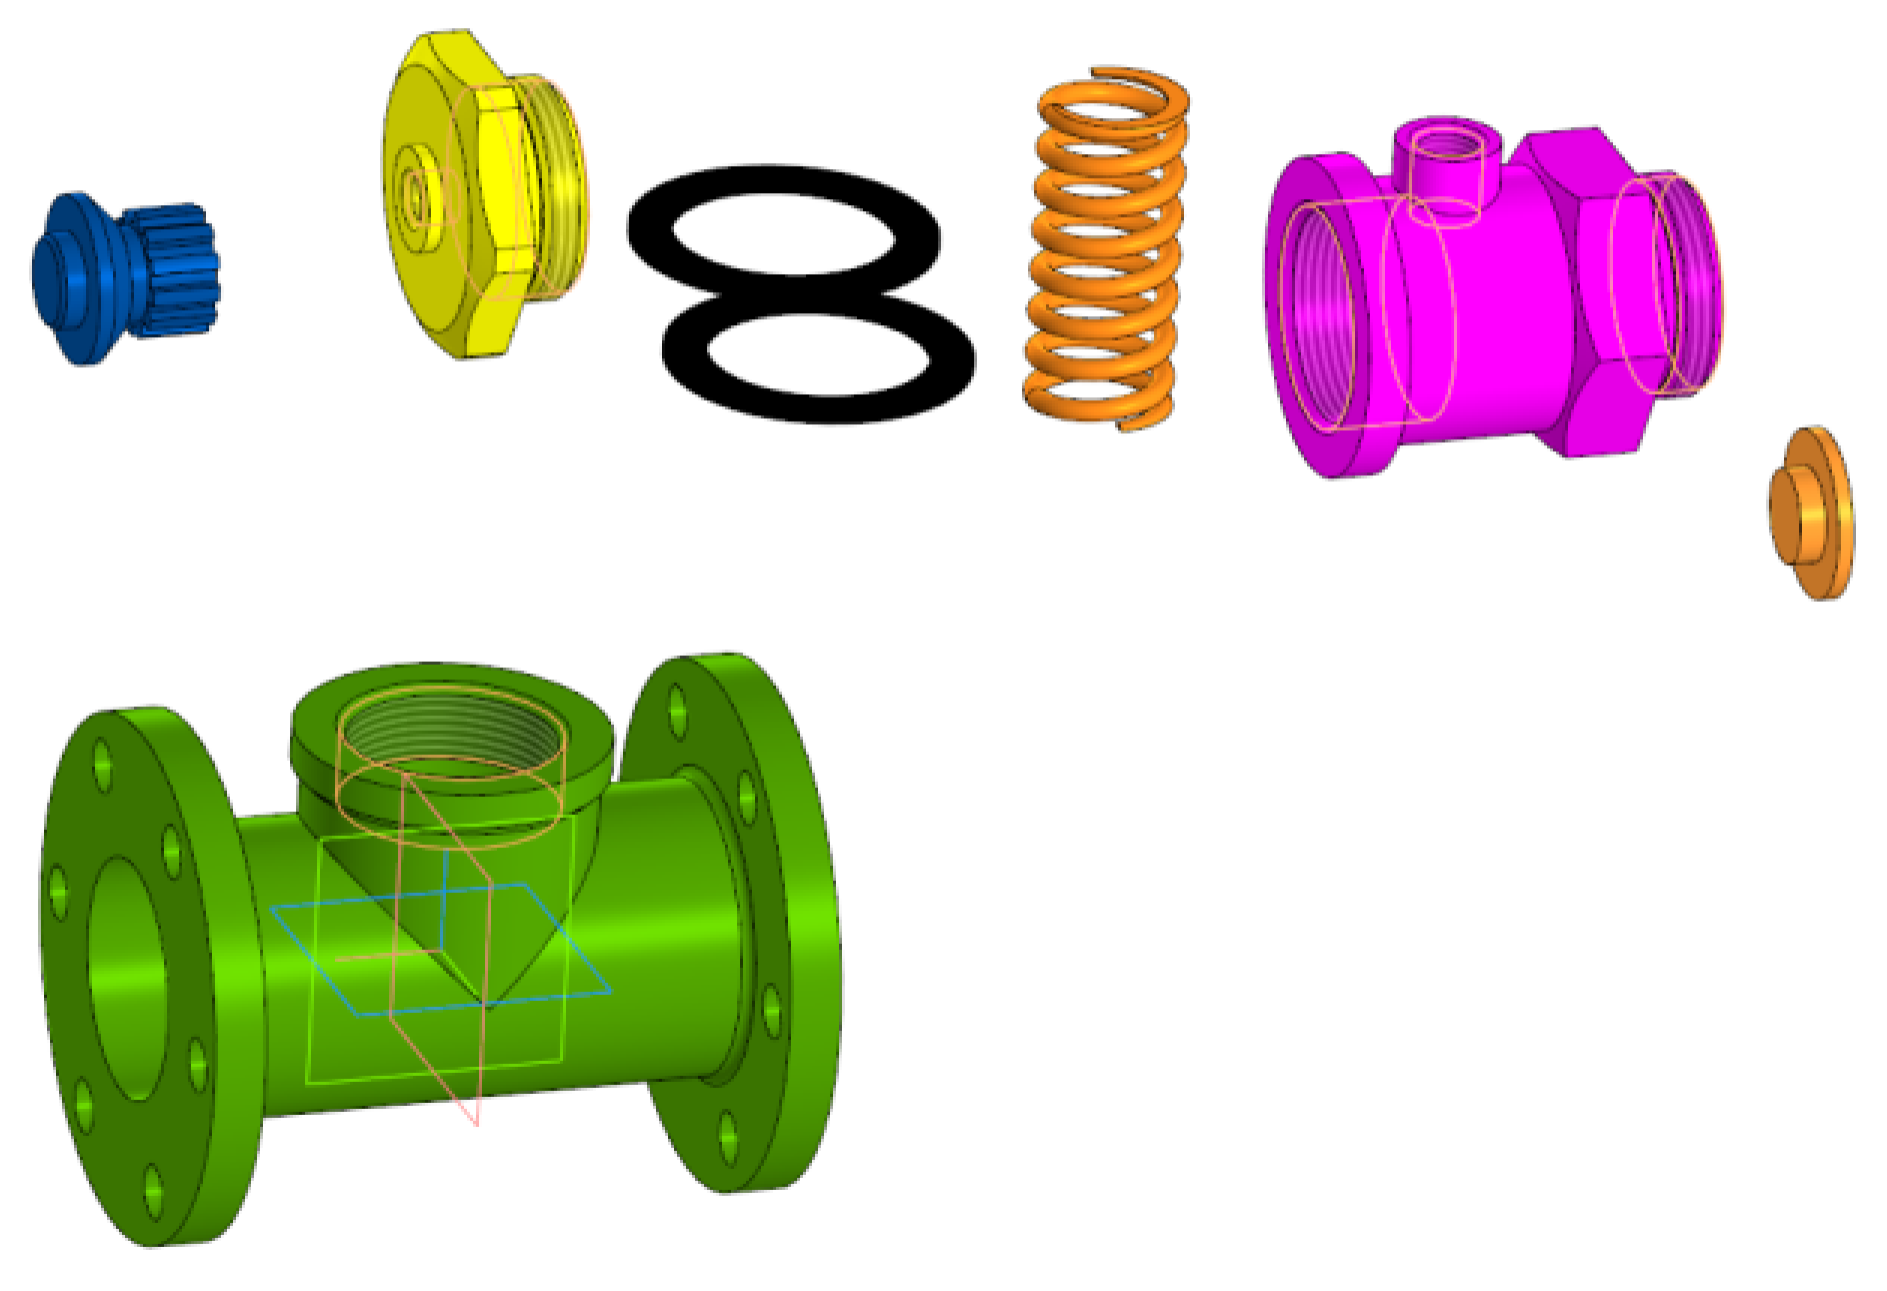
\includegraphics[height=8cm,width=1\textwidth,keepaspectratio]{resources_CAD/global_var1/h1.png}
        \caption{How it is look like in 3D}
        \label{fig:resources_CAD/global_var1/h1.png}
    \end{subfigure}

    \begin{subfigure}{0.99\textwidth}
        \centering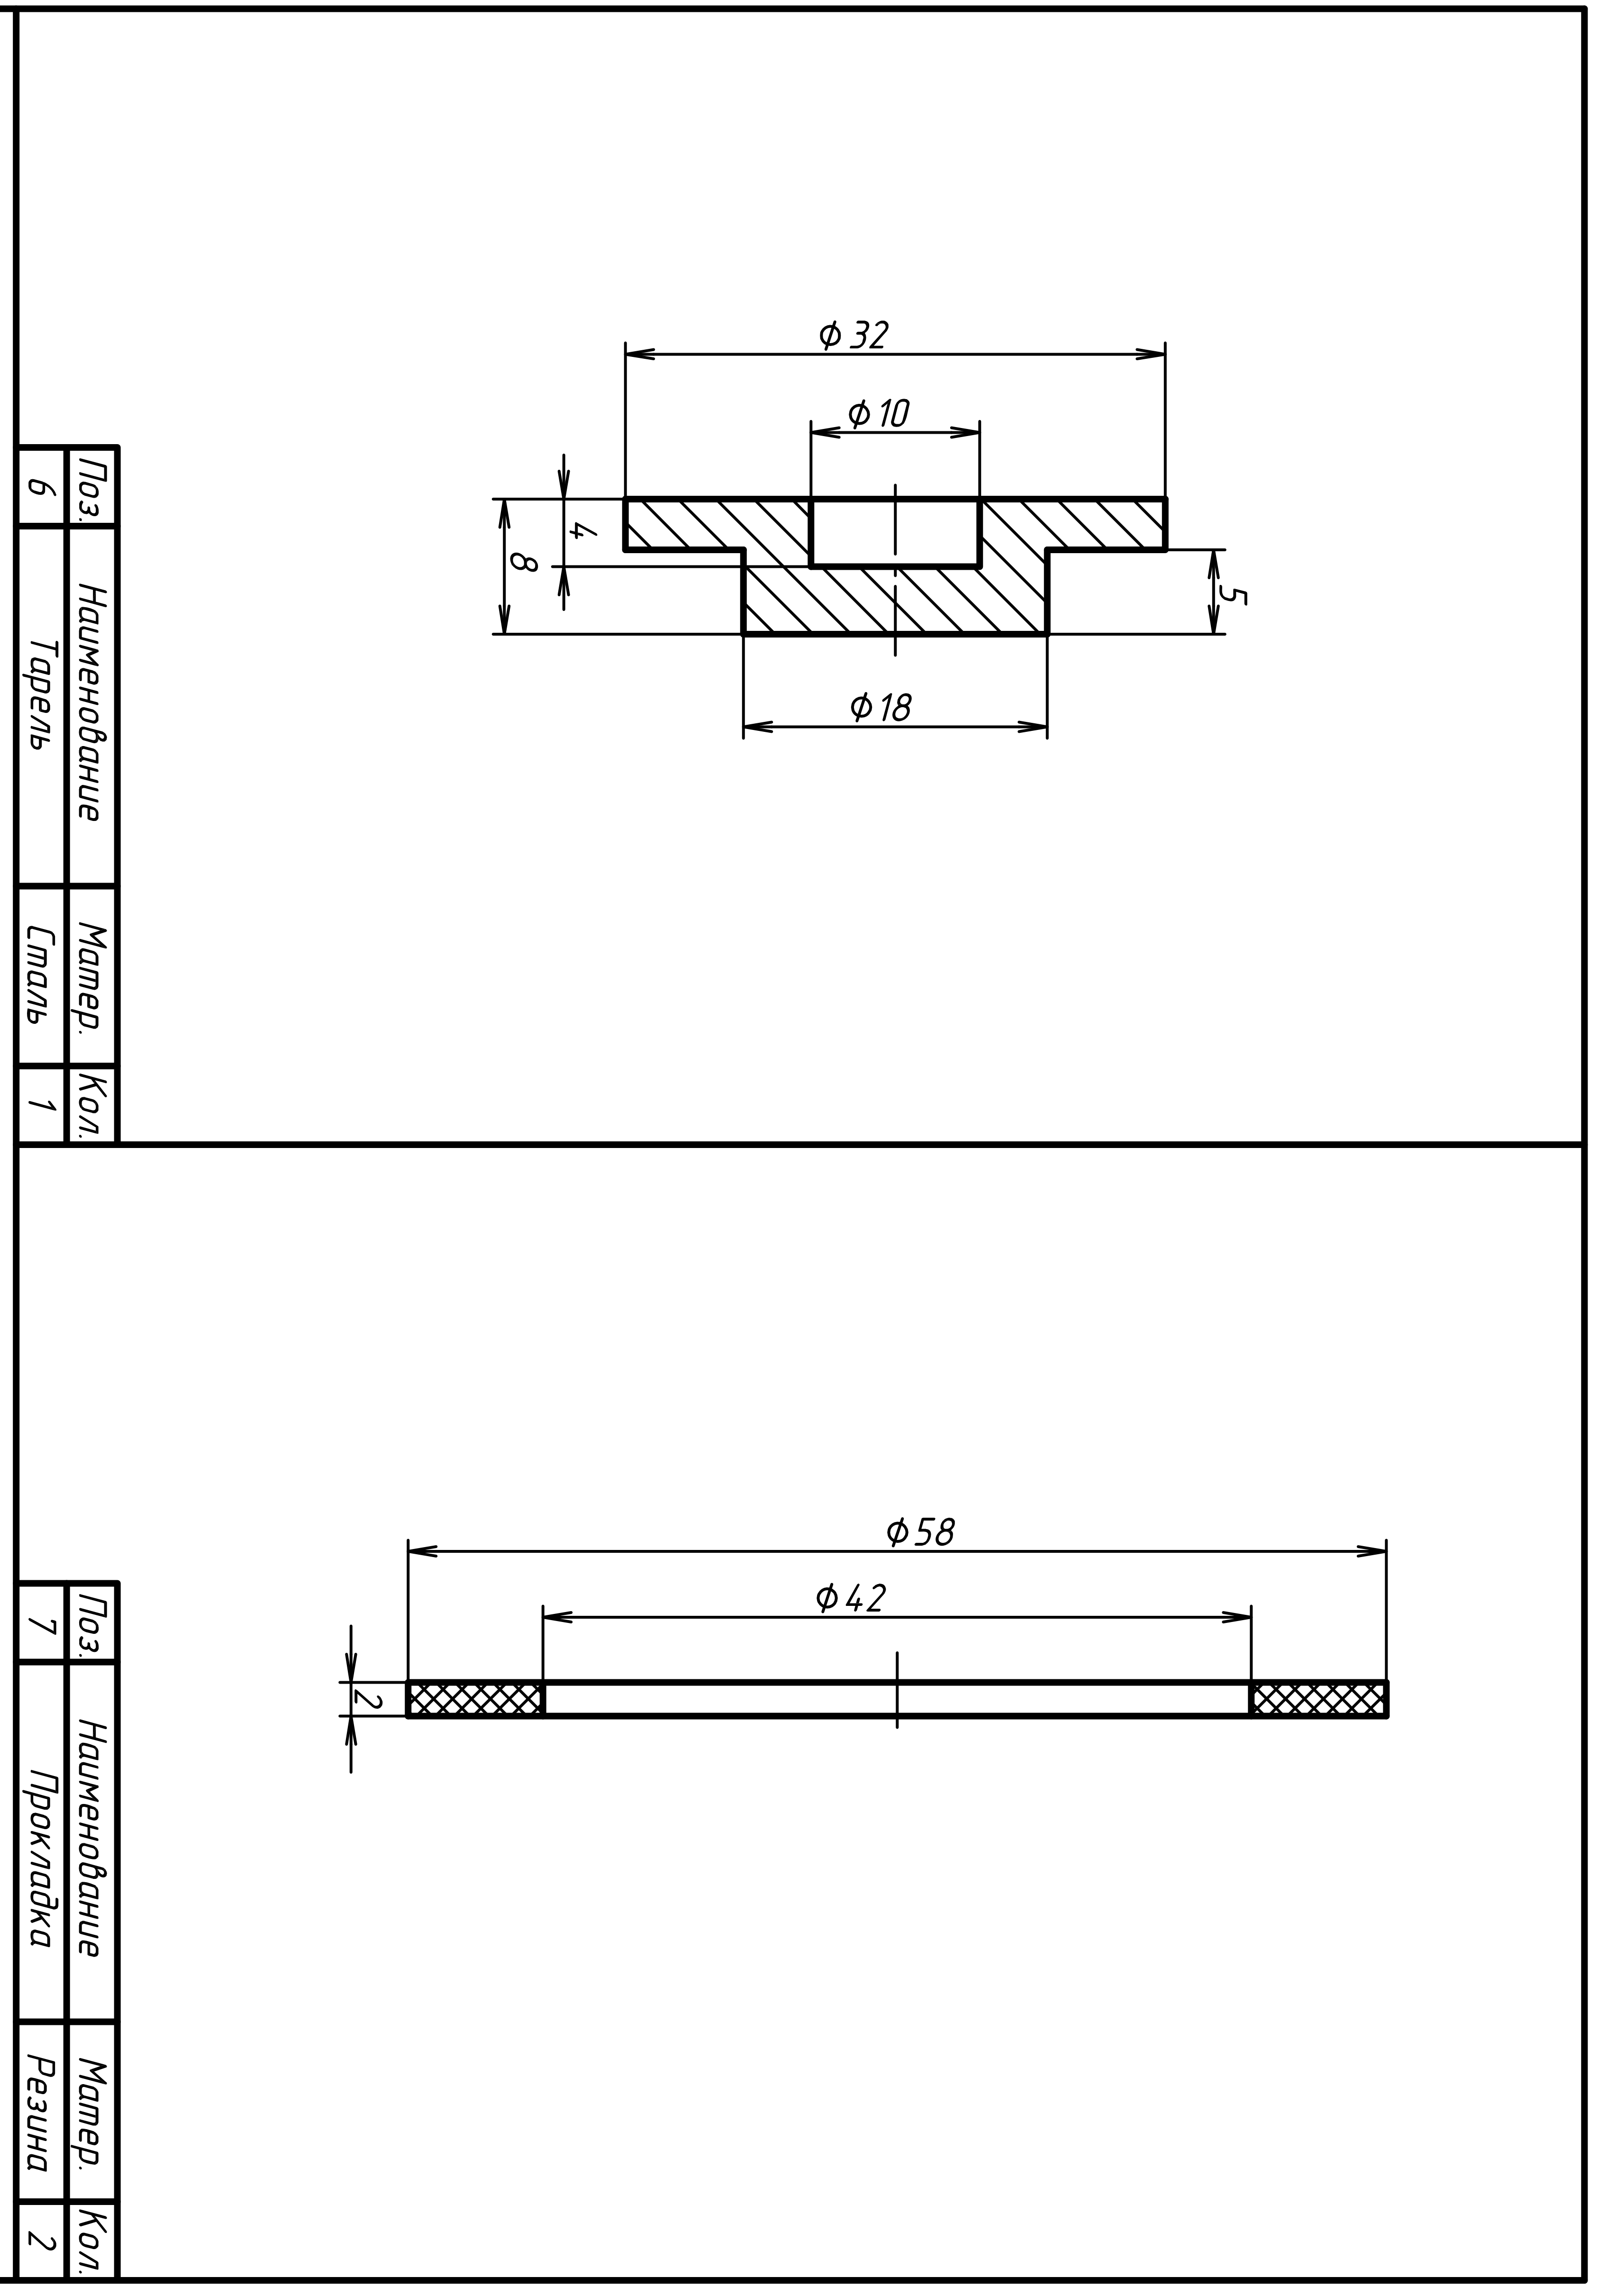
\includegraphics[height=7cm,width=1\textwidth,keepaspectratio]{resources_CAD/global_var1/t67.png}
        \caption{Parts 6 and 7}
        \label{fig:resources_CAD/global_var1/t67.png}
    \end{subfigure}

\caption{Task 1}
\label{fig:t12}
\end{figure}

\begin{figure}[H]
    \centering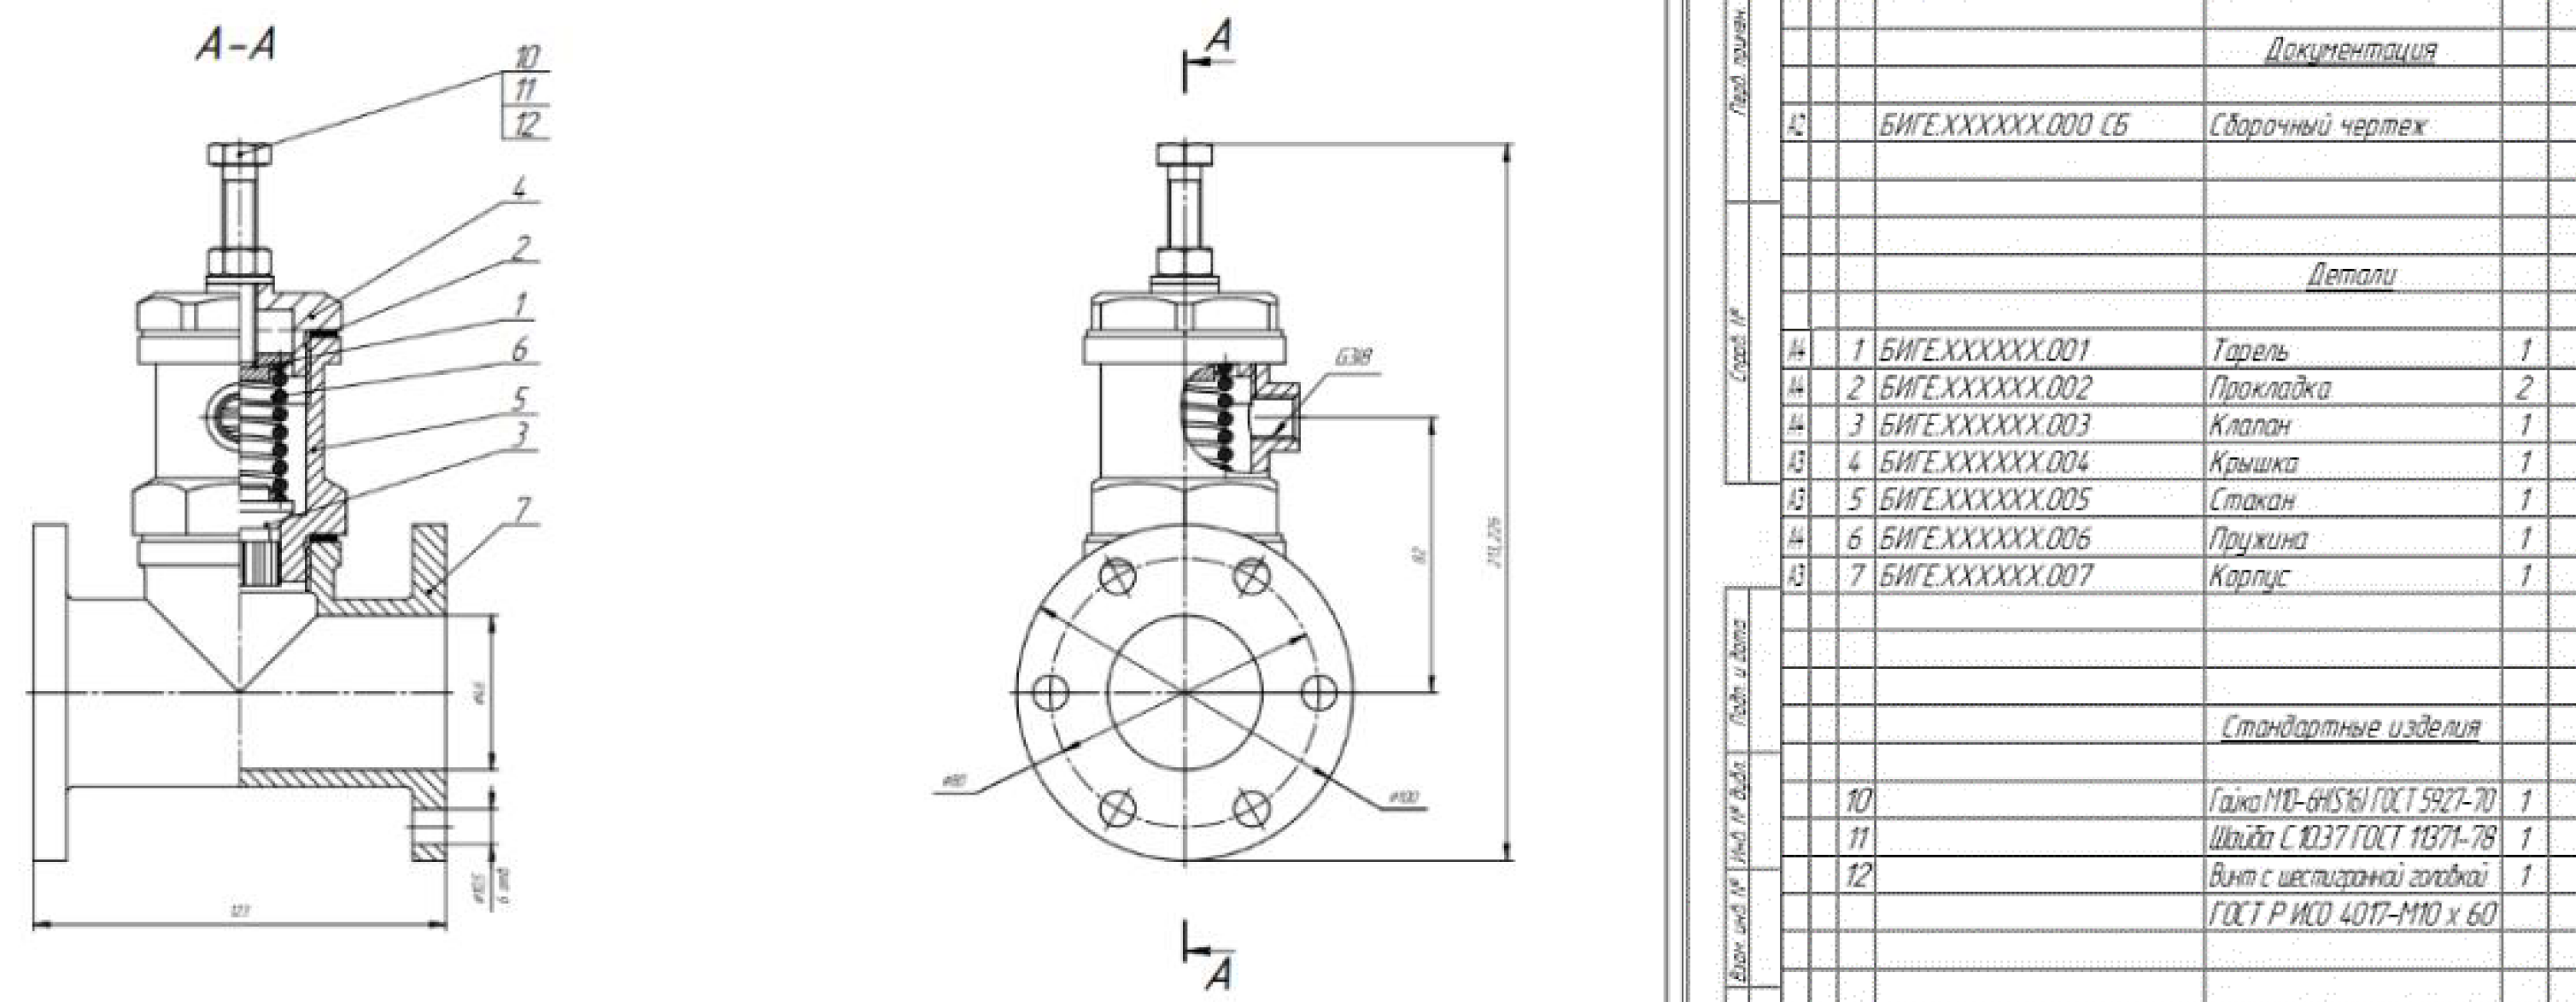
\includegraphics[height=9cm,width=1\textwidth,keepaspectratio]{resources_CAD/global_var1/h2.png}
    \caption{Task 2}
    \label{fig:resources_CAD/global_var1/h2.png}
\end{figure}
\newpage

% Global_var 2
\forloop{themenumber}{1}{\value{themenumber} < 9}{
    \begin{center}
        \LARGE <<Introduction to Mechanical Engineering>> \\ \textbf{Final Exam} \\ \textit{CAD modeling} \\ Variant: \arabic{themenumber}
    \end{center}
    \setcounter{figure}{0}
    \begin{enumerate}
        \item  Make all CAD models from the blueprints, which provided below \pic{fig:\arabic{themenumber}gt11,fig:\arabic{themenumber}gt12}. (15 score)
        \item  Make an assembly. Description is on the figure \pic{fig:\arabic{themenumber}h2.png}. (5 score)
         
        Decimal number --- <3 first surname letters>$2023.$<variant>$.000$ (Bulichev $\rightarrow$ $BUL2023.0\arabic{themenumber}.000$) 
        \item  Make the same blueprints (without dimensions), based on your CAD models. (3 extra score)
        \item  Provide a BOM for your assembly. It should contain name, decimal number, amount of details. (2 extra score)
    \end{enumerate}
    
    \begin{figure}[H]
        \begin{subfigure}{0.99\textwidth}
            \centering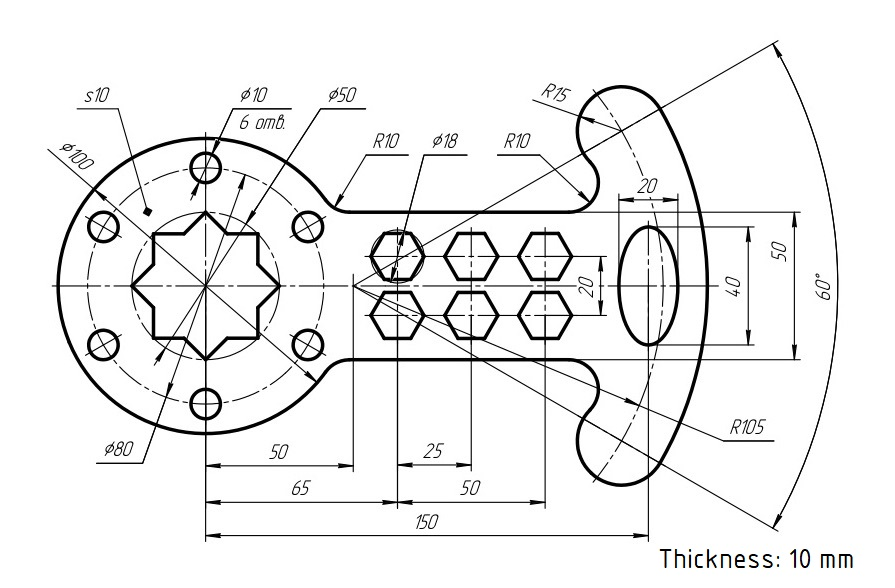
\includegraphics[height=7cm,width=1\textwidth,keepaspectratio]{resources_CAD/global_var2/t1.png}
            \caption{Part 1}
            \label{fig:resources_CAD/global_var2/t1.png}
        \end{subfigure}

        \begin{subfigure}{0.49\textwidth}
            \centering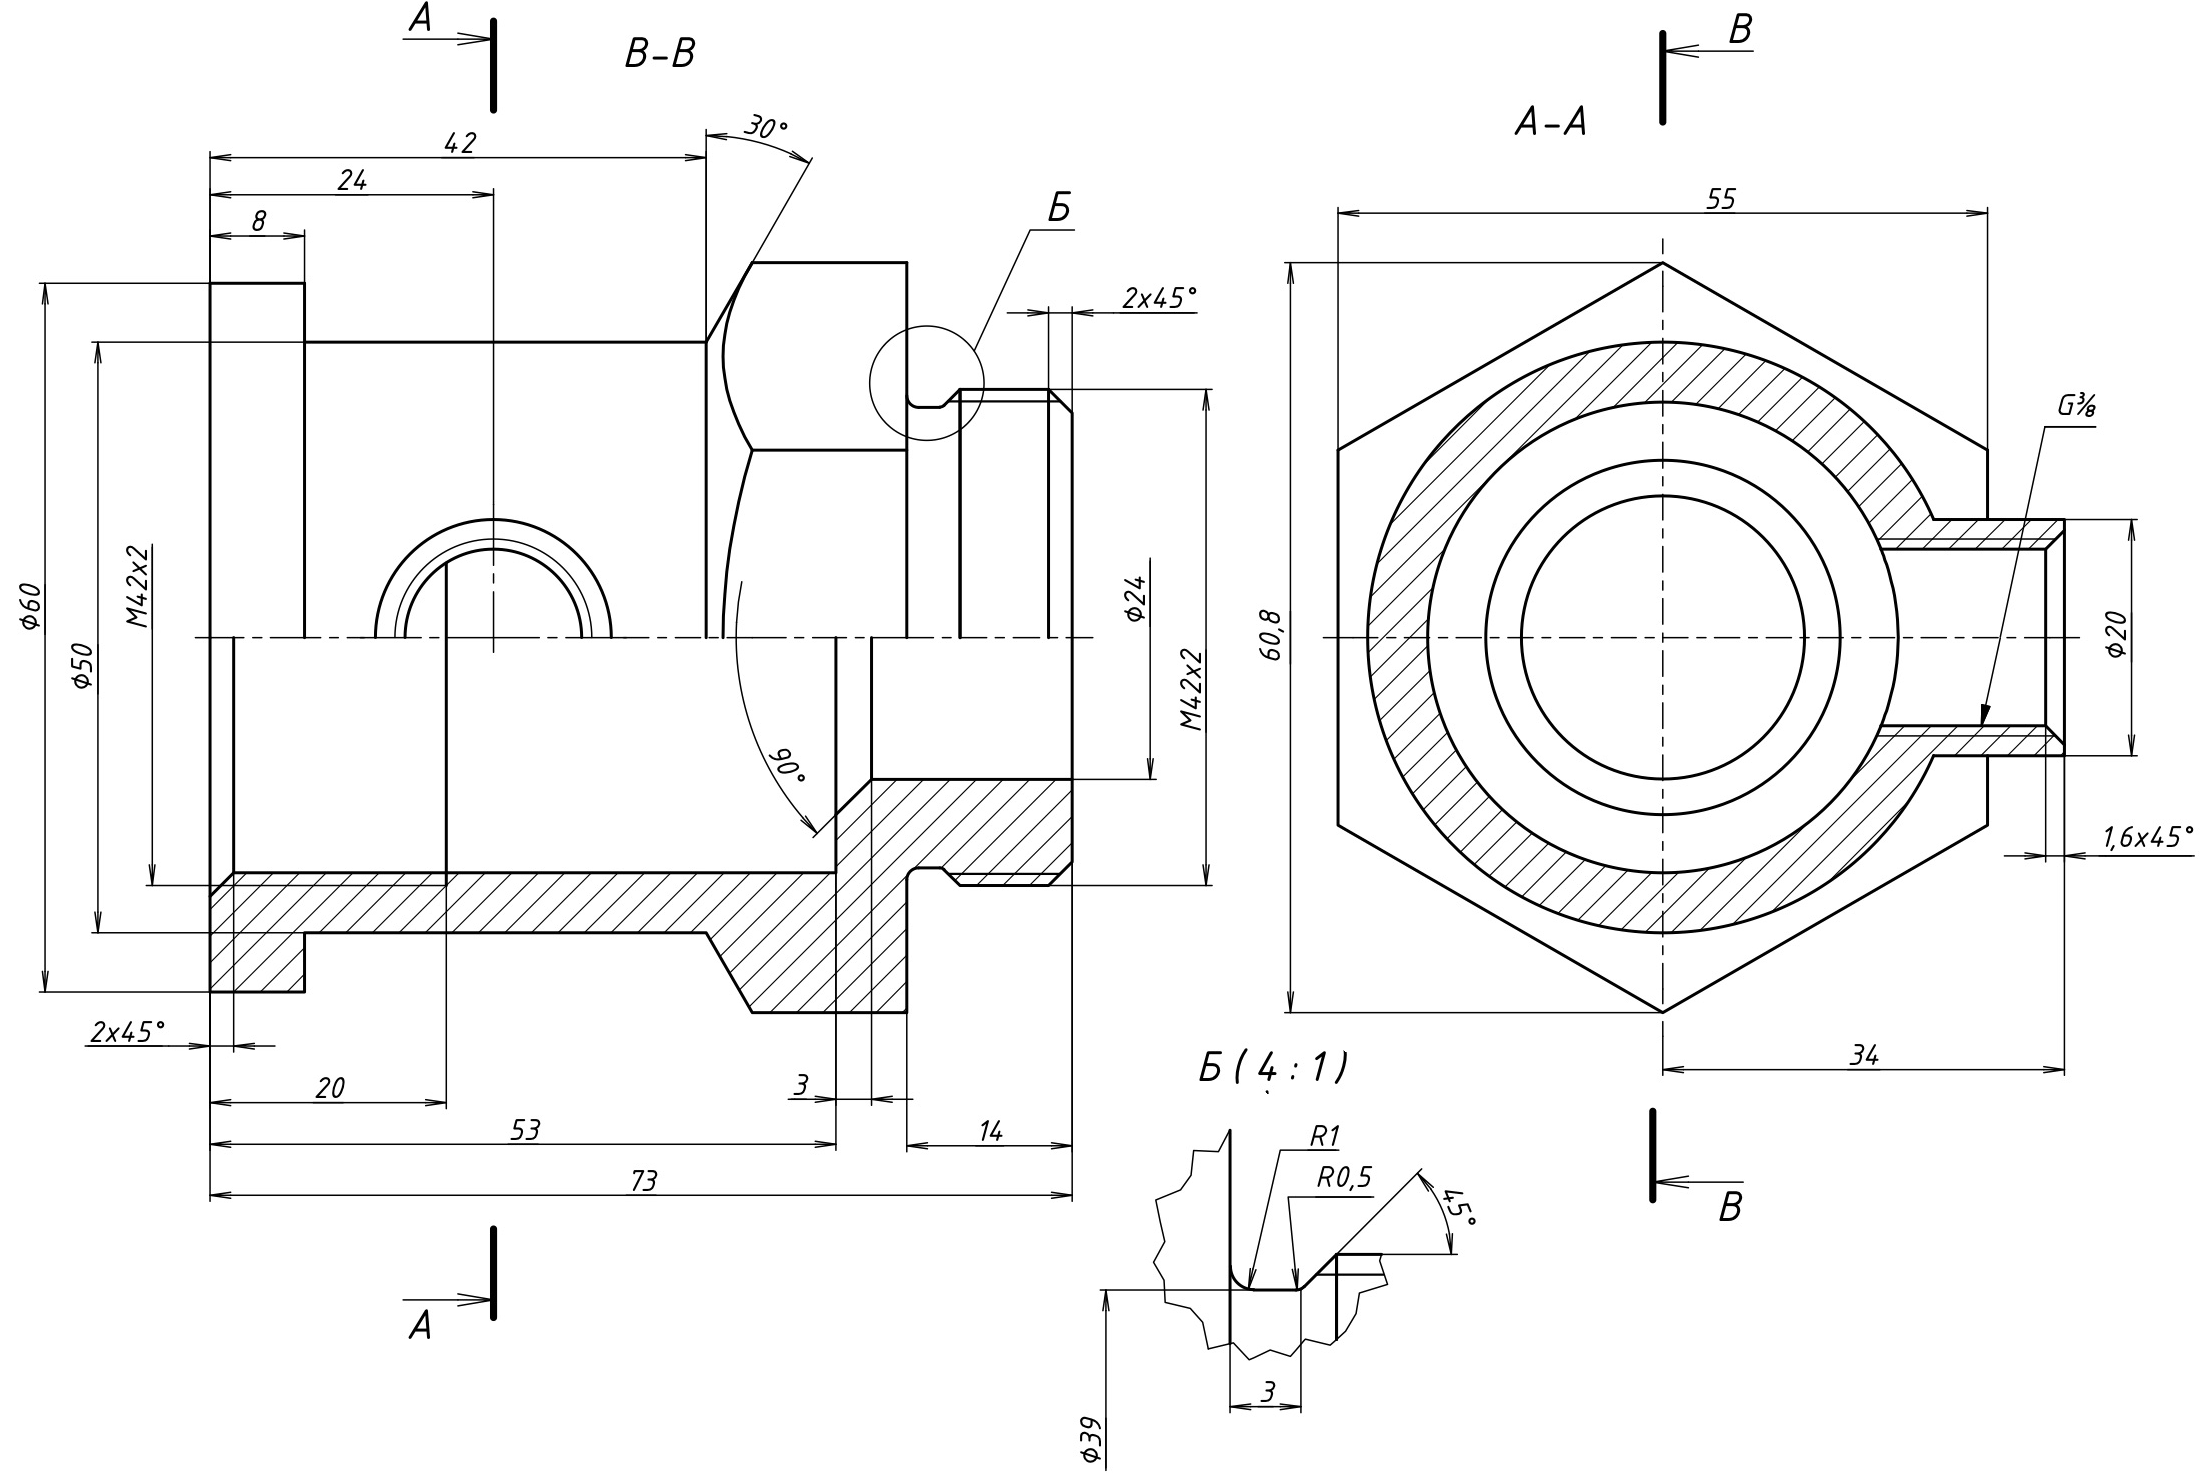
\includegraphics[height=8cm,width=1\textwidth,keepaspectratio]{resources_CAD/global_var2/t2.png}
            \caption{Part 2}
            \label{fig:resources_CAD/global_var2/t2.png}
        \end{subfigure}
        \begin{subfigure}{0.49\textwidth}
            \centering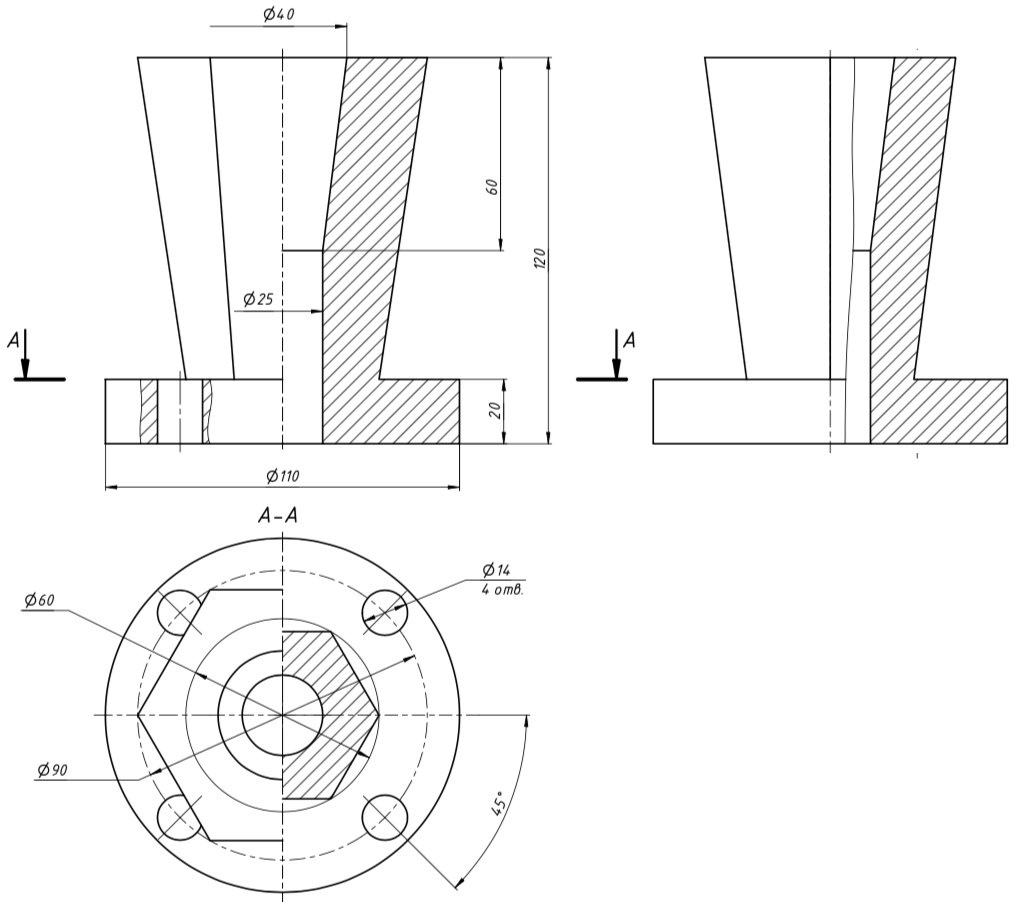
\includegraphics[height=10cm,width=1\textwidth,keepaspectratio]{resources_CAD/global_var2/t3.png}
            \caption{Part 3}
            \label{fig:resources_CAD/global_var2/t3.png}
        \end{subfigure}
    \caption{Task 1}
    \label{fig:\arabic{themenumber}gt11}
    \end{figure}
    
\begin{figure}[H]
    \begin{subfigure}{0.99\textwidth}
        \centering\includegraphics[height=8.5cm,width=1\textwidth,keepaspectratio]{resources_CAD/global_var2/var\arabic{themenumber}.png}
        \caption{Part 4}
        \label{fig:resources_CAD/global_var2/var\arabic{themenumber}.png}
    \end{subfigure}
    \begin{subfigure}{0.99\textwidth}
        \centering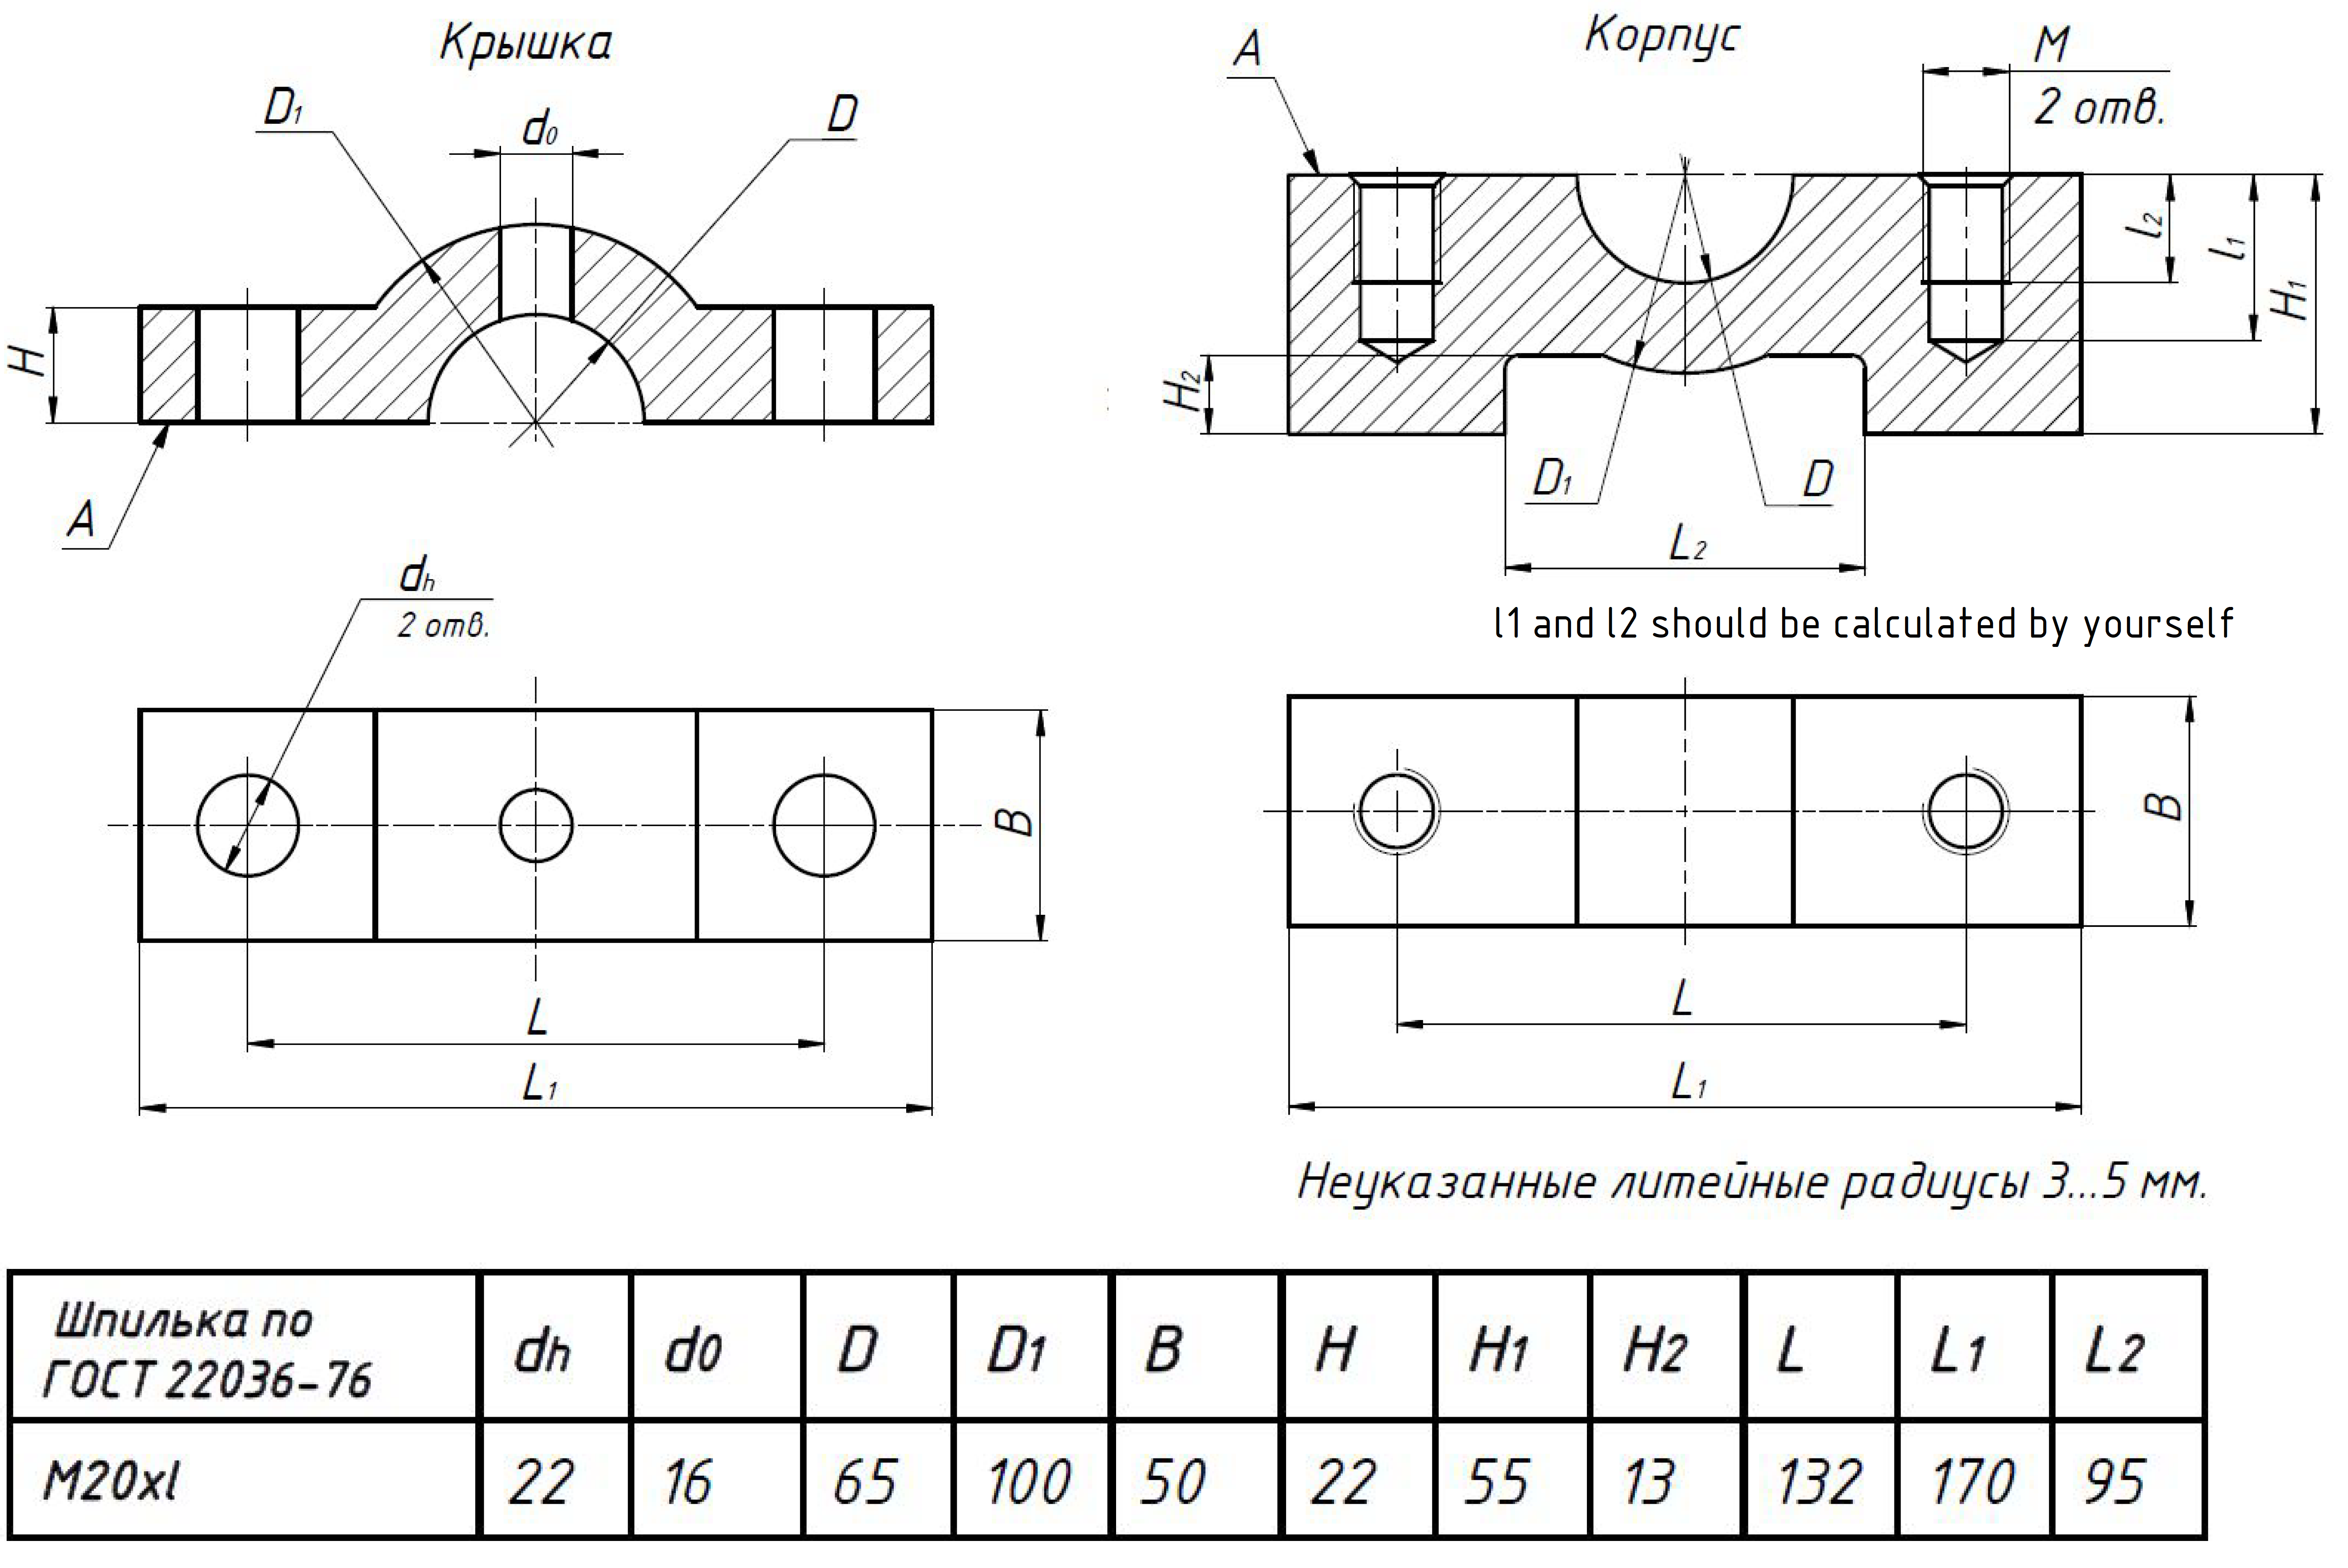
\includegraphics[height=8cm,width=1\textwidth,keepaspectratio]{resources_CAD/global_var2/t4.png}
        \caption{Parts 5 and 6}
        \label{fig:resources_CAD/global_var2/t4.png}
    \end{subfigure}

\caption{Task 1}
\label{fig:\arabic{themenumber}gt12}
\end{figure}

\begin{figure}[H]
    \centering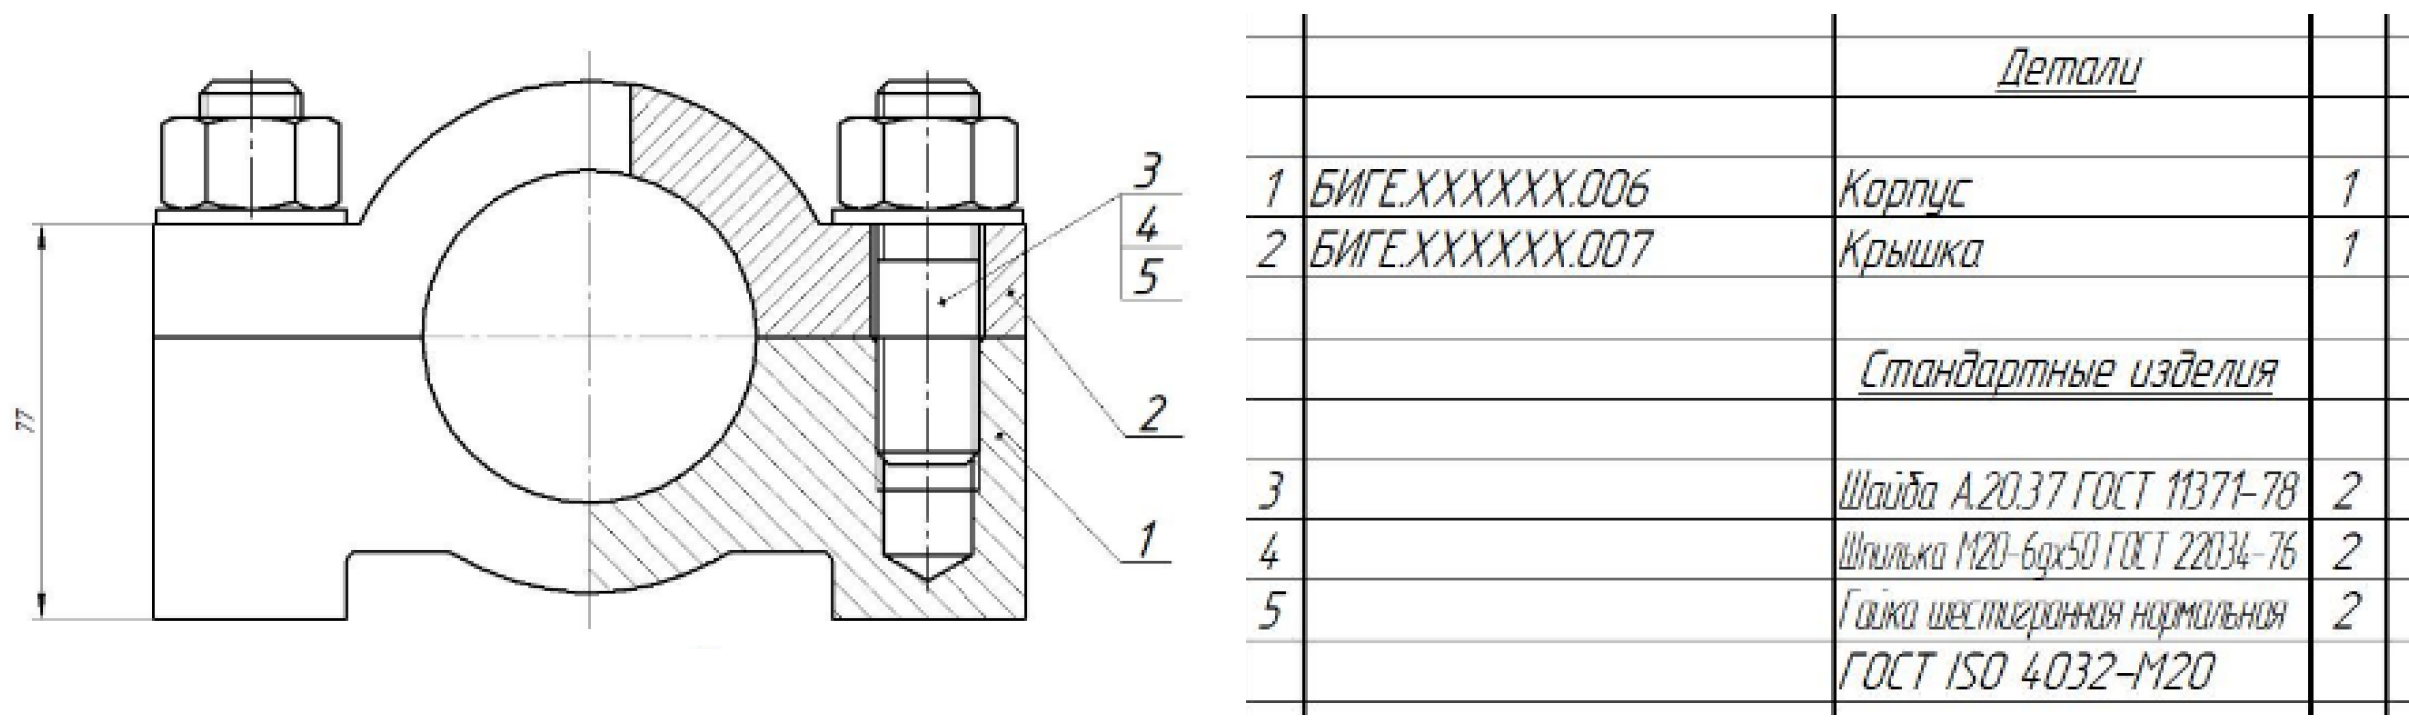
\includegraphics[height=8cm,width=1\textwidth,keepaspectratio]{resources_CAD/global_var2/h2.png}
    \caption{Task 2}
    \label{fig:\arabic{themenumber}h2.png}
\end{figure}
\newpage

}
\end{document}